%----------------------------------------------------------------
%
%  File    :  survey.tex
%
%  Author  :  Keith Andrews, ISDS, TU Graz, Austria
%
%  Created :  24 Mar 2010
%
%  Changed :  04 Mar 2019
%
%----------------------------------------------------------------


\documentclass[11pt,onecolumn,twoside]{report}
\usepackage{amsmath}
\usepackage{nccmath}


\usepackage[
  a4paper,
  twoside,
  top=5mm,                % top margin
  bottom=7mm,             % bottom margin
  inner=20mm,             % inner margin (next to binding)
  outer=20mm,             % outer margin (opposite binding)
  bindingoffset=10mm,     % on binding side
  includeheadfoot,        % include head(er) and foot(er)
  headheight=10mm,        % height of header
  headsep=15mm,           % sep between header and text body
  footskip=15mm,          % sep between body and baseline of footer
  footnotesep = 10mm plus 2mm minus 0mm  % bottom of body to top of footnote
]{geometry}
% A4 paper is w=210m, h=297mm



\newcommand{\fullh}{24cm}         % height of figures for 1 per page
\newcommand{\halfh}{9.5cm}        % height of figures for 2 per page
\newcommand{\thirdh}{6cm}         % height of figures for 3 per page


\setlength{\parindent}{1em}       % less indentation
\setlength{\parskip}{5pt plus 1pt minus 1pt}  % space before a paragraph


% \tolerance is set by LaTeX to 200
% \sloppy sets \tolerance = 9999
% which allows LaTeX more tolerance in adding word spacing

% \sloppy
% \fussy
% \tolerance = 1000

\tolerance=400 
% makes some lines with lots of white space, but      
% tends to prevent words from sticking out in the margin



\setcounter{tocdepth}{3}        % lowest section level entered in ToC
\setcounter{secnumdepth}{3}     % lowest section level still numbered




\usepackage[T1]{fontenc}        % 8-bit output chars (must be before inputenx)
\usepackage[utf8]{inputenx}     % input char encoding

\usepackage[english,austrian,british]{babel}

\usepackage{newtxtext}          % newer times fonts
\usepackage{newtxmath}

\usepackage{relsize}            % relative font sizes \smaller \larger
\usepackage{float}              % H for float placement
\usepackage{setspace}           % line spacing

\usepackage{textcomp}           % symbols such as \texttimes and \texteuro
\usepackage{latexsym}
\usepackage{fontawesome}        % fontawesome symbols

\usepackage{siunitx}            % prettier number formatting
\sisetup{%
  group-separator={,},
}
\usepackage[super]{nth}         % 1st, 2nd, 3rd, etc.

\usepackage{xspace}
\usepackage{xstring}            % string manipulation macros
\usepackage{xparse}             % commands with optional arguments
\usepackage{etoolbox}           % for \newrobustcmd
\usepackage{makecmds}           % for \makecommand
\usepackage{calc}               % for math calculations

\usepackage[svgnames,table,xcdraw]{xcolor}
\definecolor{darkgreen}{rgb}{0.0,0.2,0.0}
\definecolor{darkblue}{rgb}{0.0,0.0,0.2}
\definecolor{darkred}{rgb}{0.2,0.0,0.0}
\definecolor{verylightgrey}{gray}{0.95}
\definecolor{lightgrey}{gray}{0.9}
\definecolor{grey}{gray}{0.7}
\definecolor{black}{gray}{0.0}


\usepackage{longtable}
\usepackage{multirow}
\usepackage{tabularx}

\usepackage{verbdef}            % define robust verb strings
\usepackage{verbatim}
\usepackage{comment}



% better lists
\usepackage{enumitem}

\setlist{
  topsep=0pt,
  partopsep=0pt,
  parsep=0.6ex,
  itemsep=1.2ex,
  left=\parindent .. 2\parindent,    % bullet .. start ot text
}

\setlist[description]{
  style=sameline,
}




\usepackage{listings}                 % for listings of source code

\makeatletter
\newlength{\numwidth}%
\setlength{\numwidth}{\widthof{\normalfont{\lst@numberstyle{99}}}}% Up to 2-digit (99) line numbers
\def\lst@PlaceNumber{%
  \makebox[\numwidth+1em][l]{%
    \makebox[\numwidth][r]{\normalfont\lst@numberstyle{\thelstnumber}}%
  }%
}
\makeatother

% lstset strategy: define defaults here for
% all non-floating listings
% floated listings override these settings later

\lstset{                              % set parameters for listings
  floatplacement=tp,                  % default float placement
  numberbychapter,
  inputencoding=utf8,
  language=,                          % empty = plain text
  basicstyle=\small\ttfamily,
  tabsize=2,
  xleftmargin=2\parindent,
  xrightmargin=2\parindent,
  frame=none,
  framexleftmargin=0mm,
  rulesepcolor=\color{verylightgrey},
  numbers=none,
  numberstyle=\scriptsize,
  numbersep=2ex,
  breaklines,
  showtabs=false,
  showspaces=false,
  showstringspaces=false,
  keywordstyle=\color{black},
  commentstyle=\color{SteelBlue},
  identifierstyle=,
  stringstyle=,
  captionpos=b,
  abovecaptionskip=\abovecaptionskip,
  belowcaptionskip=\belowcaptionskip,
  extendedchars=true,
  literate=%
    {©}{{\textcopyright}}1
    {€}{{\texteuro}}1
    {Ö}{{\"O}}1
    {Ä}{{\"A}}1
    {Ü}{{\"U}}1
    {ß}{{\ss}}1
    {ö}{{\"o}}1
    {ä}{{\"a}}1
    {ü}{{\"u}}1,       % map some utf8 chars for listings
}


\lstdefinelanguage{biblatex}   % based on biblatex v 2.7a from 2013-07-14
{
  keywords={%
    @article,@book,@mvbook,@inbook,@bookinbook,@suppbook,%
    @booklet,@collection,@mvcollection,@incollection,@suppcollection,%
    @manual,@misc,@online,@patent,@periodical,@suppperiodical,%
    @proceedings,@mvproceedings,@inproceedings,@reference,@mvreference,%
    @inreference,@report,@set,@thesis,@unpublished,@xdata,%
    @conference,@electronic,@mastersthesis,@phdthesis,@techreport,@www,%
    @artwork,@audio,@bibnote,@commentary,@image,@jurisdiction,@legislation,%
    @legal,@letter,@movie,@music,@performance,@review,@software,%
    @standard,@video%
  },
  sensitive=false,
  comment=[l][\itshape]{@comment},
  morecomment=[l]{\%},
}

\lstdefinelanguage{CSS}
{
  alsoletter={-},
  morekeywords={%
  color,background,background-color,margin,padding,font,
  font-family,weight,%
  display,position,top,left,right,bottom,list,%
  style,border,size,white,space,min,width%
  },
  sensitive=false,
  morecomment=[l]{//},
  morecomment=[s]{/*}{*/},
  morestring=[b]",
}





\usepackage[compact,nobottomtitles,pagestyles,explicit]{titlesec}
% when using explicit, must explicitly include #1 for titlename

% nobottomtitles
% move section headings close to page bottom to next page
\renewcommand{\bottomtitlespace}{2cm}

% \chaptermark sets the value of \chaptertitle for later
% \@chapapp is defined as \chaptername outside the appendix,
% and as \appendixname within the appendix.
\makeatletter
\titleformat{\chapter}
[display]                                            % shape
{\chaptermark{\thechapter~~#1}\sffamily\bfseries}    % format
{\huge\@chapapp\ \thechapter}                        % label
{4ex}                                                % sep
{\Huge#1}                                            % before-code
\makeatother

\titleformat{name=\chapter,numberless}
[block]                                              % shape
{\chaptermark{#1}\sffamily\bfseries}                 % format
{}                                                   % label
{0ex}                                                % sep
{\Huge#1}                                            % before-code

\titleformat{\section}
{\normalfont\Large\sffamily\bfseries}{\thesection}{0.8em}{#1}

\titleformat{\subsection}
{\normalfont\large\sffamily\bfseries}{\thesubsection}{0.8em}{#1}

\titleformat{\subsubsection}
{\normalfont\normalsize\sffamily\bfseries}{\thesubsubsection}{0.8em}{#1}

\titleformat{\paragraph}[runin]
{\normalfont\normalsize\sffamily\bfseries}{\theparagraph}{0.8em}{#1}

\titleformat{\subparagraph}[runin]
{\normalfont\normalsize\sffamily\bfseries}{\thesubparagraph}{0.8em}{#1}


% vertical spacing before and after section titles
\titlespacing*{\section}
{0pt}{3.5ex plus 0.5ex minus 0.5ex}{0ex plus 0ex minus 0.2ex}

\titlespacing*{\subsection}
{0pt}{2.5ex plus 0.5ex minus 0.5ex}{0ex plus 0ex minus 0.2ex}

\titlespacing*{\subsubsection}
{0pt}{2ex plus 0.5ex minus 0.5ex}{0ex plus 0ex minus 0.2ex}


% define page headings how I want them

\newpagestyle{main}[\small]{
% \addtolength\headheight{6.7pt}
% \headrule
\sethead%
[{\parbox[t]{0.3\textwidth}%                    % even left
  {\sffamily\thepage}}]
[]%                                             % even centre
[{\parbox[t]{0.6\textwidth}%                    % even right
  {\raggedleft\sffamily\chaptertitle}}]
{{\parbox[t]{0.6\textwidth}%                    % odd left
  {\sffamily\sectiontitle}}}%
{}%                                             % odd centre
{{\parbox[t]{0.3\textwidth}%                    % odd right
  {\raggedleft\sffamily\thepage}}}
}



\usepackage{titletoc}

% Add extra per-chapter space to LoL to mimic LoF and LoT
% (requires package etoolbox)
\makeatletter
\patchcmd{\@chapter}% <cmd>
  {\addtocontents}% <search>
  {\addtocontents{lol}{\protect\addvspace{10\p@}}% add per-chapter space
   \addtocontents}% <replace>
  {}{}% <success><failure>
\makeatother

% Configure LoL to mimic LoF and LoT
\contentsuse{lstlisting}{lol}
\titlecontents{lstlisting}
  [3.8em]                      % left indent
  {\addvspace{1.5mm}}          % above-code per entry
  {\contentslabel{2.3em}}      % format for numbered entry
  {\hspace*{-2.3em}}           % format for unnumbered entry
  {\titlerule*[2.7mm]{.} \contentspage}  % dots and page num per entry
  []                           % below-code per entry

%\renewcommand{\lstlistlistingname}{List of Listings}





% sensible settings for floats

\setlength{\textfloatsep}{9mm plus 2mm minus 2mm}
\setlength{\floatsep}{9mm plus 2mm minus 2mm}
\setlength{\intextsep}{9mm plus 2mm minus 2mm}

\setlength{\dbltextfloatsep}{9mm plus 2mm minus 2mm}
\setlength{\dblfloatsep}{9mm plus 2mm minus 2mm}

\setlength{\abovecaptionskip}{4mm plus 2mm minus 1mm}
\setlength{\belowcaptionskip}{0mm}

% See http://www-rohan.sdsu.edu/~aty/bibliog/latex/floats.html
% See https://robjhyndman.com/hyndsight/latex-floats/

\setcounter{topnumber}{2}               % max num floats at top of page
\setcounter{dbltopnumber}{2}            % max num floats on 2col page
\setcounter{bottomnumber}{2}            % max num floats at bottom of page
\setcounter{totalnumber}{4}             % max num floats on a page

\renewcommand{\topfraction}{0.8}        % max fraction of floats at top
\renewcommand{\dbltopfraction}{0.9}     % max fraction of floats at top 2col
\renewcommand{\bottomfraction}{0.8}     % max fraction of floats at bottom
\renewcommand{\textfraction}{0.2}       % min fraction of text

% only for entirely float pages:
\renewcommand{\floatpagefraction}{0.7}      % min page fraction having floats
\renewcommand{\dblfloatpagefraction}{0.7}   % min 2col page fraction having floats


% \usepackage[section,above,below]{placeins}  % keep floats to their own section




% use caption and subfig (caption2 and subfigure are now obsolete)

\usepackage[
  position=bottom,
  margin=1cm,
  font=small,
  labelfont={bf,sf},
  format=hang,
  indention=0mm,
]{caption,subfig}

\captionsetup[subfigure]{
  margin=0pt,
  parskip=0pt,
  hangindent=0pt,
  indention=0pt,
  singlelinecheck=true,
  farskip=4mm,            % skip above subfig (assuming captions at bottom)
  captionskip=2mm,        % skip between subfig and subcaption
}


\usepackage[hyphens,obeyspaces]{url}
\def\UrlFont{\smaller\ttfamily}





\usepackage[short]{datetime}   % load datetime *after* babel, requires fmtcount
% \newdateformat{britdate}{%
% \ordinaldate{\THEDAY} \,\monthname[\THEMONTH] \THEYEAR
% }
\newdateformat{unixdate}{%
\twodigit{\THEDAY}~\shortmonthname[\THEMONTH]~\THEYEAR
}



\usepackage[
  autostyle=true,          % adapt quote style to current language
  english=british,         % british english as default
  threshold=1,             % set block quotations >1 line in display mode
  maxlevel=4,              % max nesting level
]{csquotes}

\usepackage[
  indentfirst=false,
  vskip=0pt,               % by default would be \topsep + \partopsep.
]{quoting}

% tell csquotes to use quoting environment
% for \displayquote and \blockquote
\SetBlockEnvironment{quoting}

% if cite is issued by a csquote command
\renewcommand{\mkcitation}[1]{\space#1}

% I prefer double quotes as outer
\DeclareQuoteStyle{keithbritish}%  [variant]{style}
  {\textquotedblleft}%                      opening outer mark
  {\textquotedblright}%                     closing outer mark
  [0.05em]%
  {\textquoteleft}%                         opening inner mark
  {\textquoteright}%                        closing inner mark

\ExecuteQuoteOptions{style=keithbritish}





\usepackage[
  backend=biber,
  style=ext-authoryear,        % defined in biblatex-ext package
  sorting=nyt,
  useprefix,                   % van and von are part of second name
  mergedate=false,             % only for authoryear style
  dashed=false,                % only for authoryear style
  abbreviate=false,
  maxcitenames=2,              % if > 2 authors,
  mincitenames=1,              % use first 1 then et al
  maxbibnames=99,              % if > 99 authors,
  minbibnames=6,               % use first 6 then et al
  uniquelist=minyear,
  uniquename=init,
  hyperref=true,
  backref=true,
  backrefstyle=two,
  sortlocale=en,
]{biblatex}


% set for csquotes, but \autocite only available
% after biblatex is loaded
\SetCiteCommand{\autocite}    % or maybe \parencite

% more space between entries in bib
\setlength\bibitemsep{1.5\itemsep}

% kandrews: replace round brackets with square brackets in citations
\DeclareOuterCiteDelims{parencite}{\bibopenbracket}{\bibclosebracket}
\DeclareInnerCiteDelims{textcite}{\bibopenbracket}{\bibclosebracket}

% kandrews: replace round brackets with square brackets in bibliography
% biblabeldate is a biblatex-ext feature
\DeclareFieldFormat{biblabeldate}{\mkbibbrackets{#1}}


% remove URL: from in front of URLs
\DeclareFieldFormat{url}{\url{#1}}
\DeclareFieldFormat{doi}{\doi{#1}}
\DeclareFieldFormat{isbn}{\isbn{#1}}
\DeclareFieldFormat{issn}{\issn{#1}}

% suppress urldate field
\AtEveryBibitem{\clearfield{urlyear}}

% remove In: from @article and @inproceedings entries
% https://tex.stackexchange.com/questions/10682/suppress-in-biblatex
\renewbibmacro{in:}{%
  \ifboolexpr{%
     test {\ifentrytype{article}}%
     or
     test {\ifentrytype{inproceedings}}%
  }{}{\printtext{\bibstring{in}\intitlepunct}}%
}

% make all entry titles italic
% (also removes quotation marks from around titles)
% https://tex.stackexchange.com/questions/311816/want-title-in-simple-numeric-not-italic-through-bibliography
\DeclareFieldFormat*{title}{\mkbibitalic{#1}}
\DeclareFieldFormat*{citetitle}{\mkbibitalic{#1}}

% make journal names non-italic
\DeclareFieldFormat{journaltitle}{#1\isdot}

% make proceedings names non-italic
\DeclareFieldFormat[inproceedings]{booktitle}{#1\isdot}

% use nth for edition
\DeclareFieldFormat{edition}{%
  \ifinteger{#1}
    {\nth{#1}~\bibstring{edition}}
    {#1\isdot}}

% overwrite some standard strings in english.lbx
\DefineBibliographyStrings{english}{%
  edition          = {Edition},
  mathesis         = {Master's Thesis},
  phdthesis        = {PhD\addabbrvspace Thesis},
}


% kandrews
% use Unix format for dates in biblio:
% 29 Dec 2015, 01 Oct 2018, etc.

% for now, define under lang english not british
% due to bug in biblatex 3.11

\DefineBibliographyStrings{english}{%
  january          = {Jan},
  february         = {Feb},
  march            = {Mar},
  april            = {Apr},
  may              = {May},
  june             = {Jun},
  july             = {Jul},
  august           = {Aug},
  september        = {Sep},
  october          = {Oct},
  november         = {Nov},
  december         = {Dec},
}

\DefineBibliographyExtras{english}{%
% #1 = year, #2 = month, #3 = day
\protected\def\mkbibdatelong#1#2#3{%
  \iffieldundef{#3}
    {}
    {\mkdayzeros{\thefield{#3}}%
     \iffieldundef{#2}{}{\nobreakspace}}%
  \iffieldundef{#2}
    {}
    {\mkbibmonth{\thefield{#2}}%
     \iffieldundef{#1}{}{\space}}%
  \iffieldbibstring{#1}{\bibstring{\thefield{#1}}}{\mkyearzeros{\thefield{#1}}}}%
%
\protected\def\mkbibdateshort#1#2#3{%
  \iffieldundef{#3}
    {}
    {\mkdayzeros{\thefield{#3}}%
     \iffieldundef{#2}{}{\nobreakspace}}%
  \iffieldundef{#2}
    {}
    {\mkbibmonth{\thefield{#2}}%
     \iffieldundef{#1}{}{\space}}%
  \iffieldbibstring{#1}{\bibstring{\thefield{#1}}}{\mkyearzeros{\thefield{#1}}}}%
}


% patch for biblatex 3.11 issue with babel .lbx files
% https://github.com/plk/biblatex/issues/742
% should no longer be necessary with biblatex 3.12
\makeatletter
\protected\long\def\blx@lbx@input@handler@simple#1#2#3#4#5#6{%
  \blx@info@noline{Trying to load #2..}%
  \IfFileExists{#1}
    {\blx@info@noline{... file '#1' found}%
     #3\@@input\@filef@und#4#5%
     \ifcsundef{blx@file@lbx@simple@#1}
       {\listxadd\blx@list@req@stat{#1}%
        \@addtofilelist{#1}%
        \global\cslet{blx@file@lbx@simple@#1}\@empty}
       {}}
    {\blx@info@noline{... file '#1' not found}#6}}

\protected\long\def\blx@lbx@input@handler@once#1#2#3#4#5#6{%
  \ifcsundef{blx@file@lbx@once@#1}
    {\blx@info@noline{Trying to load #2..}%
     \IfFileExists{#1}
       {\blx@info@noline{... file '#1' found}%
        #3\@@input\@filef@und#4#5%
        \ifcsundef{blx@file@lbx@simple@#1}
          {\listxadd\blx@list@req@stat{#1}%
           \@addtofilelist{#1}}
          {}}
       {\blx@info@noline{... file '#1' not found}#6}%
     \global\cslet{blx@file@lbx@once@#1}\@empty
     \global\cslet{blx@file@lbx@simple@#1}\@empty}
    {#5}}
\makeatother


\addbibresource{resp-tables.bib}

% adapt pdftitle, pdfsubject, pdfauthor, pdfkeywords
% for your survey paper

\usepackage{ifpdf}

\ifpdf
  % pdflatex
  \usepackage[pdftex]{graphicx}
  \DeclareGraphicsExtensions{.pdf,.jpg,.png}
  \pdfcompresslevel=9
  \pdfpageheight=297mm
  \pdfpagewidth=210mm
  \usepackage[         % hyperref should be last package loaded
    unicode,
    pdftex,
    pdfversion=1.7,
    pdftitle={Writing a Survey Paper},
    pdfsubject={Survey Paper Template},
    pdfauthor={Keith Andrews},
    pdfkeywords={survey paper, skeleton, guidelines, template},
    bookmarks,
    bookmarksnumbered,
    linktocpage,
    colorlinks,
    linkcolor=darkred,
    anchorcolor=red,
    citecolor=darkgreen,
    urlcolor=darkblue,
    pdfview={Fit},
    pdfstartview={Fit},
    pdfpagemode=UseOutlines,       % open bookmarks in Acrobat
    plainpages=false,              % avoids duplicate page number problem
    pdfpagelabels,                 % avoids duplicate page number problem
    breaklinks=true,               % allow links exceeding a single line
  ]{hyperref}

\else
  % latex
  \usepackage[dvips]{graphicx}
  \usepackage[dvips]{hyperref}
  \DeclareGraphicsExtensions{.eps}
\fi



% subset of macros from thesis-macros

% \liintro list item intro is a style used when list items have an
% introduction phrase (say in italics) followed by a colon.
\newcommand{\liintro}[1]{\emph{#1}}

% short notes in square brackets
\newcommand{\shortnote}[1]
{%
{{\smaller{}[#1]}}
}


\newcommand{\TODO}[1]
{
{\textcolor{red}{[TODO: #1]}}
}



\newcommand{\imgcredit}[1]
{\smaller{}[#1]}



\newcommand{\copyrightACM}
{%
Copyright \copyright\ by the Association for Computing Machinery, Inc.%
}




\newcommand{\daymonthyear}[3]
{%
\twodigit{#1}\hspace{0.7ex}\nolinebreak[2]\shortmonthname[#2]\hspace{0.7ex}\nolinebreak[2]#3%
}


\newcommand{\monthyear}[2]
{%
\shortmonthname[#1]\hspace{0.7ex}\nolinebreak[2]#2%
}


\newcommand{\yearmonthday}[3]
{%
\twodigit{#3}\hspace{0.7ex}\nolinebreak[2]\shortmonthname[#2]\hspace{0.7ex}\nolinebreak[2]#1%
}


\newcommand{\yearmonth}[2]
{%
\shortmonthname[#2]\hspace{0.7ex}\nolinebreak[2]#1%
}



% link to Amazon or
% http://worldcatlibraries.org/wcpa/isbn/[ISBN number]
% http://amazon.com/exec/obidos/ASIN/#1/keithandrewshcic
% http://amazon.com/dp/#1/

\newrobustcmd{\isbn}[1]
{%
{%
\ifpdf
{\smaller ISBN
\href{http://amazon.co.uk/dp/#1/}{#1}}%
\else
{\smaller ISBN #1}%
\fi
}%
}



% ISSN
% http://www.bl.uk/services/bibliographic/issn.html
% 8 digits, should be printed xxxx-xxxx
% e.g. 0020-0190 is Information Processing Letters, Elsevier
%
% Lookup services:
% http://kmittlib.lib.kmutt.ac.th:81/search/i?SEARCH=0020-0190
% http://worldcatlibraries.org/wcpa/issn/0020-0190

\newrobustcmd{\issn}[1]
{%
{%
\ifpdf
{\smaller ISSN
\href{http://worldcatlibraries.org/wcpa/issn/#1}{#1}}%
\else
{\smaller ISSN #1}%
\fi
}%
}



% DOIs  http://doi.org/  e.g.
% doi:10.1038/nature723
% http://doi.org/10.1038/nature723

\newrobustcmd{\doi}[1]
{%
{%
\def\UrlFont{\smaller\rmfamily}
\ifpdf                                   % pdflatex
\href{http://doi.org/#1}{doi:\protect\nolinkurl{#1}}%
\else                                    % latex
doi:\protect\nolinkurl{#1}%
\fi
}%
}





\newrobustcmd{\website}[1]
{%
\ifpdf                                  % pdflatex
\href{http://#1/}{\nolinkurl{#1}}%
\else                                   % latex
\nolinkurl{#1}%
\fi
}




\newcommand{\news}[1]
{%
\ifpdf
\href{news:#1}{\nolinkurl{#1}}
\else
\nolinkurl{#1}%
\fi
}








% based on url package
% define styles for class, file, and variable names
% which break nicely at line breaks

% make the macros robust so they work inside captions, etc

\newcommand{\ttname}{\begingroup \smaller\urlstyle{tt}\Url}
\newcommand{\rmname}{\begingroup \smaller\urlstyle{rm}\Url}
\newcommand{\sfname}{\begingroup \smaller\urlstyle{sf}\Url}


% fname is for file names and directory names
\newrobustcmd{\fname}[1]{\ttname{#1}}

% vname is for variable names, domain names, email addresses
\newrobustcmd{\vname}[1]{\ttname{#1}}




% for class names, define our own url style

\makeatletter  % protect @ names

% \url@letstyle: New URL style to premit break at any letters.
% Based on \url@ttstyle

\def\Url@letdo{% style assignments for tt fonts or T1 encoding
\def\UrlBreaks{\do\a\do\b\do\c\do\d\do\e\do\f\do\g\do\h\do\i\do\j\do\k\do\l%
               \do\m\do\n\do\o\do\p\do\q\do\r\do\s\do\t\do\u\do\v\do\w\do\x%
               \do\y\do\z%
               \do\A\do\B\do\C\do\D\do\E\do\F\do\G\do\H\do\I\do\J\do\K\do\L%
               \do\M\do\N\do\O\do\P\do\Q\do\R\do\S\do\T\do\U\do\V\do\W\do\X%
               \do\Y\do\Z%
}%
\def\UrlBigBreaks{\do\.\do\@\do\\\do\/\do\!\do\_\do\|\do\%\do\;\do\>\do\]%
 \do\)\do\,\do\?\do\'\do\+\do\=\do\#\do\:\do@url@hyp}%
\def\UrlNoBreaks{\do\(\do\[\do\{\do\<}% (unnecessary)
\def\UrlSpecials{\do\ {\ }}%
\def\UrlOrds{\do\*\do\-\do\~}% any ordinary characters that aren't usually
\Urlmuskip = 0mu plus 1mu%
}

\def\url@letstyle{%
\@ifundefined{selectfont}{\def\UrlFont{\sf}}{\def\UrlFont{\sffamily}}\Url@letdo
}

\makeatother  % unprotect @ names

% class names
\newcommand\letname{\begingroup \smaller\urlstyle{let}\Url}

\newrobustcmd{\cname}[1]{\letname{#1}}






% Euro symbol
\newcommand{\euro}{\texteuro\,}

% times symbol
\newcommand{\timessym}{\texttimes\,}

% approx symbol
\newcommand{\approxsym}{\ensuremath\approx\,}

% plusminus symbol
\newcommand{\plusminussym}{\textpm\,}

% not equal symbol
\newcommand{\neqsym}{\ensuremath{\neq\,}}

% rightarrow symbol
\newcommand{\rightarrowsym}{\ensuremath\rightarrow\,\,}


% thumbs up and thumbs down symbols

\newcommand{\uthumb}{\smaller[2]\raisebox{1pt}{\textcolor{DarkGreen}{\faThumbsUp}}}

\newcommand{\dthumb}{\smaller[2]\raisebox{1pt}{\textcolor{DarkRed}{\faThumbsDown}}}







\begin{document}

\unixdate

\normalsize
\pagestyle{empty}         % for preliminary pages (no numbers shown)
\pagenumbering{Roman}     % for pdf labels




\begin{titlepage}

\begin{center}
\begin{spacing}{1.1}
\Large\sffamily\bfseries
Responsive Web Tables
\end{spacing}

\vspace{1cm}

{\large\sffamily Mirza Kabiljagic, Stefan Rajinovic, Aleksandar Stojicic, Inti Gabriel Mendoza Estrada}

% {\large\sffamily Group 4}
% \vspace{5mm}
% {\large\sffamily Keith Andrews, Tom Strong, Bill Weak, and Seb Green}

\vspace{1cm}

Institute of Interactive Systems and Data Science (ISDS), \\
Graz University of Technology \\
A-8010 Graz, Austria \\[1cm]


% {\large
% 706.057 Information Visualisation SS 2019 \\
% Graz University of Technology \\[1cm]
% }

\vspace{1cm}

{29 Nov 2019}

\end{center}



\vspace{2cm}

\begin{quote}
\begin{center}
{\large\sffamily\bfseries Abstract}
\end{center}
Responsive techniques are techniques used in web design which enable better rendering of web pages, tables, and other elements. With better rendering, it is meant as a rescaling of the resolution of the device used to open the specific website. When using responsive techniques, it doesn't matter which device is used to look at a website, the website should look good. 


It is mostly a combination of fluid grids, which enables the elements of a page to be sized in relative units, such as percentages, rather than using pixels or points, flexible images, same thing as in fluid grids, media queries, which enable using many CSS tricks or style rules and responsive layout which can automatically adapt, resize, and adjust to any device screen size, be it a laptop, mobile phone or tablet.


Responsive tables are tables which use the approach mentioned above, which allow them to be more flexible and complex, without compromising its usability while adding a better aesthetically pleasing look. In this survey report, we will provide a good overview of what responsive techniques, responsive tables, and good table designs are, and, finally, recommend the best technique combination, in our opinion, to use. 

\end{quote}

\vfill

\begin{center}
{\footnotesize\sffamily \copyright ~ Copyright 2019 by the author(s),
except as otherwise noted.}

\vspace{2mm}
{\footnotesize\sffamily This work is placed under a
Creative Commons Attribution 4.0 International
(\href{https://creativecommons.org/licenses/by/4.0/}{CC BY 4.0}) licence.}
\end{center}

\end{titlepage}




\cleardoublepage
\pagestyle{plain}             % for preliminary pages
\pagenumbering{roman}         % for preliminary pages


\begin{spacing}{0.8}
\tableofcontents
\end{spacing}
\addcontentsline{toc}{chapter}{Contents}

\cleardoublepage
\begin{spacing}{0.8}
\listoffigures
\end{spacing}
\addcontentsline{toc}{chapter}{List of Figures}

%\cleardoublepage
%\begin{spacing}{0.8}
%\listoftables
%\end{spacing}
%\addcontentsline{toc}{chapter}{List of Tables}

%\cleardoublepage
%\begin{spacing}{0.8}
%\renewcommand{\lstlistlistingname}{List of Listings}
%\lstlistoflistings
%\end{spacing}
%\addcontentsline{toc}{chapter}{List of Listings}



\cleardoublepage
\pagestyle{main}              % for main pages
\pagenumbering{arabic}        % for main pages


\cleardoublepage  
%----------------------------------------------------------------
%
%  File    :  survey-intro.tex
%
%  Author  :  Keith Andrews, IICM, TU Graz, Austria
% 
%  Created :  27 May 1993
% 
%  Changed :  16 Nov 2010
% 
%----------------------------------------------------------------


\chapter{Introduction}

\label{chap:Intro}

Going back, at the starting point of web development, its creators
and designers have not had the need to think about the look and design
of the page, because back then, their users and clients would mostly access
the site via the same device, that being a personal desktop computer which would
mostly share the same resolution and display size. That means that they mostly
needed to design and work around the same concept. Also, they didn’t need to think
about things like what if an user entered the site with this device or this, so
they could basically use static and fixed positioning of elements.

However, todays' technologies, be it the mobile industry or technical industry
in general, the devices have come a long way, and are being worked on really
fast. What does that mean is that the programmers and designers need 
to consider that people will have different ways of using and browsing their 
pages, which require different approaches to design their web pages.
Nowadays, the clients and users have a broad list of devices, which they can use
to access a web page, be it a tablet, mobile phone, laptop and even TVs[1][2].    

Basically, the most important thing is to make the web pages' user interface 
as friendly as possible, so that the user does not lose much time navigating around.
And with that being said, web programmers need to automatically think about
making the web pages in that way, while they are being accessed from those different
devices mentioned[2].

Responsive Web Design is an approach, or more rather a technique, which is used
to construct a self-adapting web page, meaning that it adapts, resizes, shrink
and changes its' form in any way needed to perfectly fit the web-accessing device
used to visit it[3].   





\section{How to achieve Responsive Web Design}

If a programmer wants his web site to be responsive, he has to use 
following techniques:

$\bullet$ Media queries 

$\bullet$ Flexible images and media

$\bullet$ Fluid grid layouts



\section{Media queries}

Media queries are very important because with them it is possible to specify 
with what device the web page is being accessed. The query usually is made of
a media type, and some conditions which can check if the media type has some special
property.
\\
\\
\begin{lstlisting}[%
    language = CSS, 
    float=tp,
    xleftmargin=0cm,              % no extra margins for floats
    xrightmargin=0cm,             % no extra margins for floats
    language=biblatex,
    basicstyle=\footnotesize\ttfamily,
    frame=shadowbox,
    numbers=left,
    label=list:BibACMIEEE,
    ,
]
    % An example of a media query, where one can say that for a screen of size 850px or less, the background is black:

    @media screen and (max-width: 600px) {
    body   {
          background-color: olive;
        }
    }
\end{lstlisting}
Basically it allows defining specific CSS rules, depending on the device used.

From this example above, with the help of the parameter \emph{screen}
the media type was specified and using \emph{max-width} the condition was determined which
affects the device of the user. Now, there are many different conditions which
can be used, and they are really helpful, because with them it is possible to adjust 
display settings for every device there is. 

For example, if the user is entering the website with his phone, it can be automatically said that an image should have a lower resolution,
thus adjusting it better for his screen and saving some bandwith.

Another example would be using \emph{display:none} with which some content can completely be hidden that should not be 
displayed.

\begin{lstlisting}[%
    language = HTML, 
    xleftmargin=0cm,              % no extra margins for floats
    xrightmargin=0cm,             % no extra margins for floats
    language=biblatex,
    basicstyle=\footnotesize\ttfamily,
    frame=shadowbox,
    numbers=left,
    label=list:BibACMIEEE,
     stringstyle=\color{blue}
    ,
]
    % An example of using display: none:

    <!DOCTYPE html>
    <html>
    <head>
    <style>
    h1.none {
      display: none;
    }
    </style>
    </head>
    <body>

    <h1 class="none">This will not be displayed</h1>

    </body>
    </html>

\end{lstlisting}




%
If this was ran in the browser, header would not be seen, because
it was decided to not be shown. If \emph{display:none} was changed to \emph{display:block}
our header would be visible.

Include a list of \emph{all} the relevant papers and resources you
have found and mark those you have chosen to focus on. Make sure
\emph{all} the papers and resources you found or were given appear in
the bibliography.




\section{Fluid Grid Layouts}

Normally, websites are constructed in a layout which is grid-built, because they are
easier to handle in different kind of devices. Also what is specific
for that kind of layout is that it is built using divs, HTML tables and so on. Now, on top of that
responsive web design comes in play[5]. With it, it is possible to use percentage-based element sizing which is easier than using pixels. 

According by (Abdulrehman,2015) a flexible grid-layout is one of the foundations of responsive
design. Using the term "grid" does not mean necessarily that a grid framework needs to be used.
What it means is that specific CSS tricks are used for positioning. Also, he suggest that 
using pixels for the measurement unit should be stopped, because pixels can vary. 

For example, on one device they can be one point or dot, on another device it can be a few more, and therefore
unreliable. So, what needs to be done is that, if pixels are used, they should be converted using
a formula stated by (Marcotte, 2010) in  Dan Cederholm's book named "Handcrafted CSS":

\begin{ceqn}
\begin{align}
    Target \div Context = Result
\end{align}
\end{ceqn}

It is asserted by (Pettit, 2012) that, to use this formula, the context of the element
needs to be divided by the target element.
%TODO -> Example and how to achieve/use Fluid Grid Mirza



\section{Flexible images and media}

With this approach, any type of media,images depending on the screen resolution
will resize,collapse,crop and adjust accordingly to it, and to achieve this
it is possible to use the same thing mentioned in the previous section, relative units,
if the screen becomes too small then hide the image completely or by cropping some parts
of the image, again in the case if the screen becomes too small[6].

\subsection{Relative measurements} 

Instead of using pixels,relative dimensions can be used, percentage based. So instead of
specifying the view and dimensions in pixels, one can specify for example 60\%, which would result
in resizing or reshrinking of the image based on the resolution of the device accordingly to fill
60\% of the page. 

%\begin{figure}[h!]
  %  \centering
  %  \includegraphics[keepaspectratio,width=\linewidth,height=\halfh]
  %  {relative.png}
    
  %  \caption[Relative Image]{
  %  The web site of the TeX Users Group \parencite{TUG}.
    
   % \label{fig:TUG}
    %\end{figure}
    \begin{figure}[h!]
        \centering
        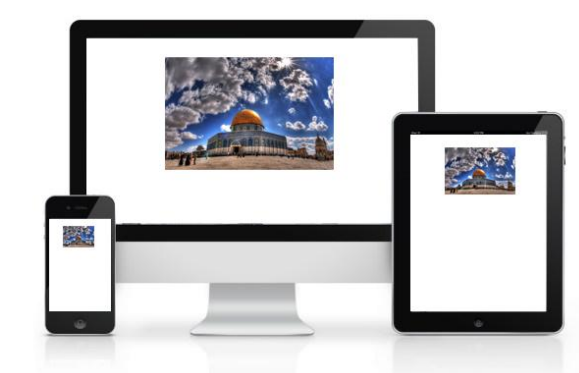
\includegraphics[keepaspectratio,width=\linewidth,height=\halfh]
        {relative.png}
        
        \caption[Relative Image Dimensions]{
            Relative Image Dimensions.
        \imgcredit{Taken from research paper.}
        }
        \label{fig:TUG}
        \end{figure}
%TODO SPECIFY LINK AL NE RADI MAMU MU
\newpage
\subsection{Cropping} 

Another option is cropping, which crops the picture to a certain width
with the help of CSS. 

\begin{figure}[h!]
    \centering
    \subfloat[%  the % chars remove implicit spacing
    Picture with original size
    ]
    {%
    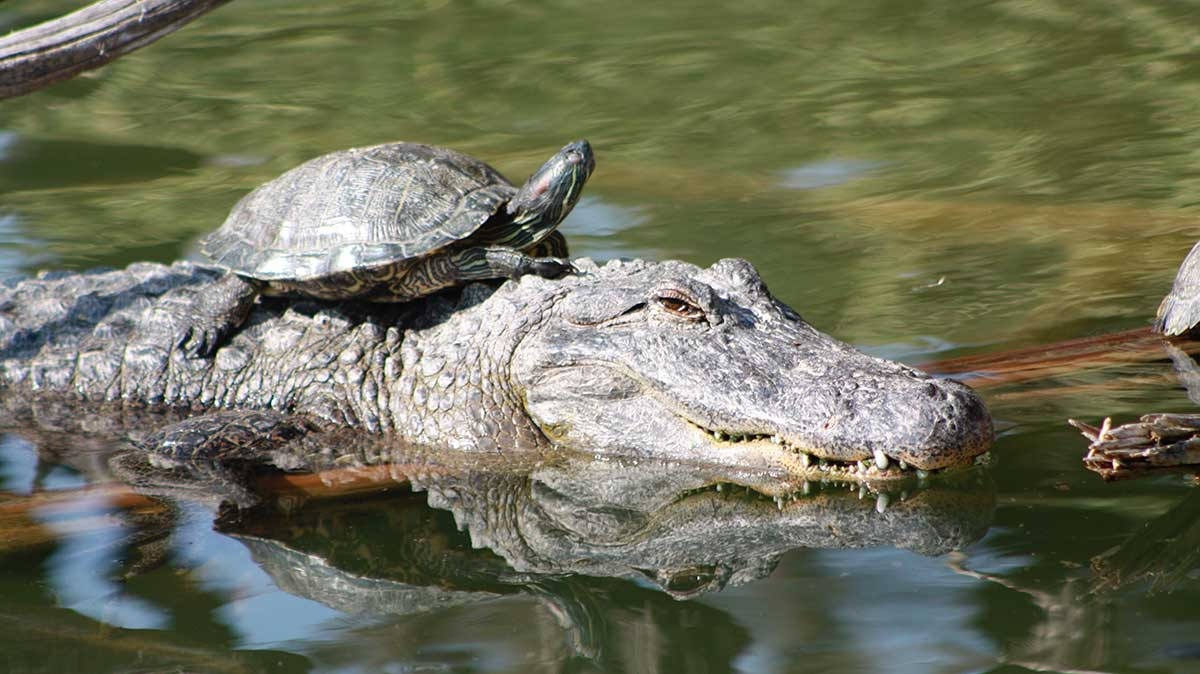
\includegraphics[width=\linewidth]
    {alig1.jpg}%
    \label{alig1}%
    }
    \hfill
    \subfloat[%
    Picture when cropped 
    ]
    {%
    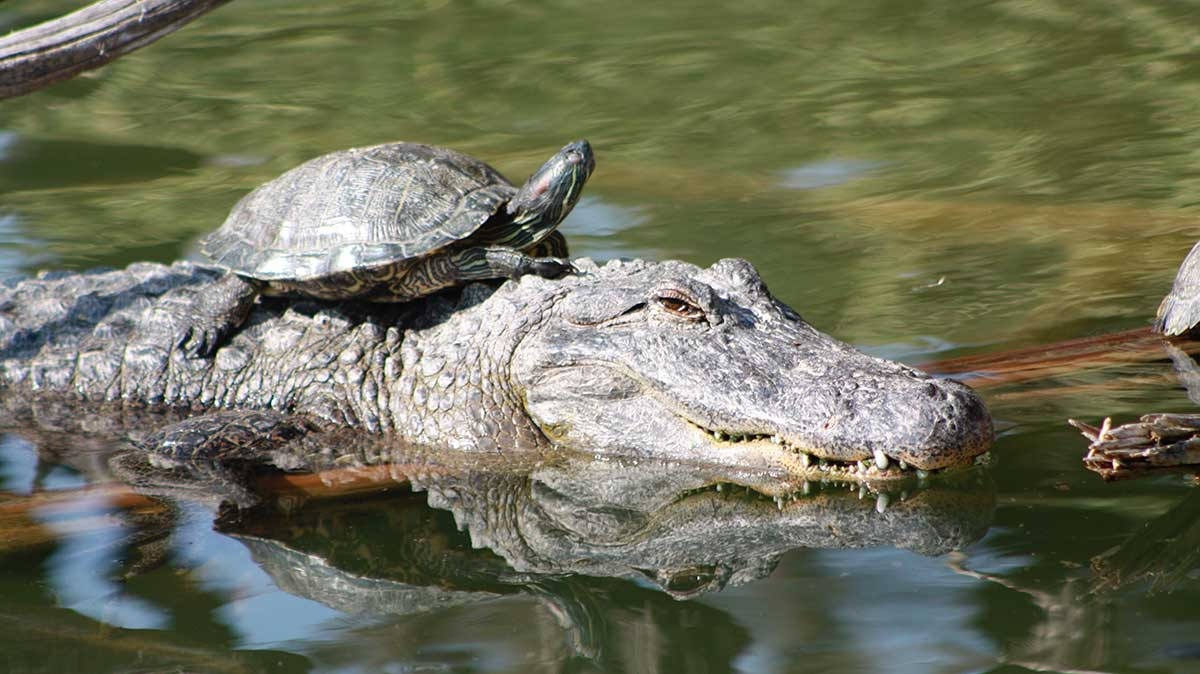
\includegraphics[width=0.45\linewidth]
    {alig2.jpg}%
    \label{alig2}%
    }
    
    \caption[Image Cropping]
    {
      Image cropping.
    \imgcredit{https://alligator.io/css/cropping-images-object-fit/.}
    }
    \label{figWhol}
\end{figure}

In this Figure above, it can be obviously seen that the result of tweaking the image a bit.
With just a few CSS commands, it is possible to crop the picture and if someone is browsing the
web site with a smaller device, the image does not have to be hidden, just its' size is changed.

\begin{lstlisting}[%
    language = HTML, 
    xleftmargin=0cm,              % no extra margins for floats
    xrightmargin=0cm,             % no extra margins for floats
    language=biblatex,
    basicstyle=\footnotesize\ttfamily,
    frame=shadowbox,
    numbers=left,
    label=list:BibACMIEEE,
     stringstyle=\color{blue}
    ,
]
    % An example of a media query, where one can say that for a screen of size 850px or less, the background is black:

    figure{
     width:300px; /*container-width*/
     overflow:hidden; /*hide bounds of image */
     margin:0;   /*reset margin of figure tag*/
   }
   figure img{
     display:block; /*remove inline-block spaces*/
     width:100%; /*make image streatch*/
}
\end{lstlisting}
Taken from
\imgcredit{https://medium.com/@elad/how-to-crop-images-with-css-b8471d402b16.}   

\cleardoublepage
%----------------------------------------------------------------
%
%  File    :  survey-browsers.tex
%
%  Author  :  Keith Andrews, IICM, TU Graz, Austria
%
%  Created :  27 May 1993
%
%  Changed :  16 Nov 2010
%
%----------------------------------------------------------------


\chapter{HTML Tables}

\label{HTML5 Tables}

In case of having much data to display, or data which is better of in a grid, HTML tables
are the best solution available. Before, tables have been used mostly for the layout of
HTML web-sites and it is not a good practice to do so, mainly because of two things:


$\bullet$ Semantically it is wrong

$\bullet$ Tables aren't as adaptable and flexible as divs'

\section{Structure of tables}

The basic structure of an HTML table starts with the \textit{<table>} tag. It is the starting
point for constructing a table. Now, HTML tables consist of columns and rows, like normal
tables. For rows, the tag  \textit{<tr>} is used, whereas for table header \textit{<th>} tag
is used. Normally, table headers are positioned in the center and are bold. For table cells
\textit{<td>} tag is used \parencite{7}.
\newpage

\begin{lstlisting}[%
    language = CSS,
    xleftmargin=0cm,              % no extra margins for floats
    xrightmargin=0cm,             % no extra margins for floats
    language=biblatex,
    basicstyle=\footnotesize\ttfamily,
    frame=shadowbox,
    numbers=left,
    label=list:BibACMIEEE,
    ,
]
    % An example of an HTML Table which demonstrates information about cars:
    <!DOCTYPE html>
<html>
<head>
	<title>Best Cars 2019</title>
</head>
<body>
<table class="table table-bordered table-hover table-condensed">
	<thead>
		<tr>
			<th title="Field #1">Car</th>
			<th title="Field #2">Manufacturer</th>
			<th title="Field #3">Engine Size</th>
			<th title="Field #4">Cylinders</th>
			<th title="Field #5">Horsepower</th>
			<th title="Field #6">Torque</th>
			<th title="Field #7">Compresion Ratio</th>
			<th title="Field #8">Miles per gallon</th>
			<th title="Field #9">Price</th>
		</tr>
	</thead>
	<tbody>
		<tr>
			<td>2019 Acura RDX</td>
			<td>Acura</td>
			<td>2.00L</td>
			<td align="right">4</td>
			<td align="right">272</td>
			<td align="right">280</td>
			<td>9.8:1</td>
			<td align="right">28</td>
			<td>€33,600.00</td>
		</tr>
		<tr>
			<td>2019 Ford Ranger</td>
			<td>Ford</td>
			<td>2.30L</td>
			<td align="right">4</td>
			<td align="right">270</td>
			<td align="right">310</td>
			<td>10.0:1</td>
			<td align="right">21</td>
			<td>€21,800.00</td>
		</tr>
	</tbody>
</table>

</body>
</html>

\end{lstlisting}

Now, there exist some other tags which can be used for HTML5 tables:

$\bullet$ <thead> - Table header, it is used to point out single or multiple rows
of a table, which do not contain table data but column labels \parencite{8}.

$\bullet$ <tbody> - Table body, it is used to point out <tr> elements. Position this tag
always after <thead>, but it can also come after or before <tfoot> \parencite{8}.

$\bullet$ <tfoot> - Table footer, it is used to point out single or multiple <tr> elements
where those elements are presenting an overview  of the data in the table \parencite{8}.

$\bullet$ <caption> - Table caption, as the name already says, can be used to specify table caption.
Can be put on the bottom of the CSS document.

$\bullet$ <col> - While using col and some other keyword, for example, align, it is possible direct
the alignment of text in the table. There are other keywords whom can be used to adjust colors, width
and many other things of table columns.





\section{Good Table Design}
Now, there are certain guidelines which can help a developer, or if that person can be called that way,
table maintainer, make a table and its design better. By that is meant that there are some interesting ways
where a little of simple CSS can be used to your advantage to make your table stand out.


\subsection{Alternate row highlighting}
When presented a table with a lot of entries, it can be hard to look at. Scrolling through numerous rows can be frustrating.
With this CSS trick, it can be a bit easier, atleast for the eyes if nothing else. The idea is to color every even row, while leaving
the odd ones in tact.
As said, it is pretty simple, and requires only two lines of CSS, but also pretty useful.


\begin{lstlisting}[%
    language = HTML,
    xleftmargin=0cm,              % no extra margins for floats
    xrightmargin=0cm,             % no extra margins for floats
    language=biblatex,
    basicstyle=\footnotesize\ttfamily,
    frame=shadowbox,
    numbers=left,
    label=list:BibACMIEEE,
     stringstyle=\color{blue}
    ,
]
    % An example of using simple CSS to color table rows:

	table.alt tr:nth-child(even) {background: #CCC}
	table.alt tr:nth-child(odd) {background: #FFF}

\end{lstlisting}


And now, at the end, this is the final result:
\begin{figure}[H]
    \centering

    {%
    \includegraphics[width=\linewidth]
    {alt_t.jpeg}%
    \label{alig1}%
    }


    \caption[Alternate row highlighting]
    {

    \imgcredit{Screenshot taken by the author.}
    }
    \label{figWhol}
\end{figure}


\newpage
\subsection{Current Row Highlighting}
Now again, talking about a big table, and going through it, one may
easily becomes lost and wouldn't know in which row he is at the moment, which can be
pretty stressful. Again with the help of some CSS, the lives of the users' is made easier.

\begin{lstlisting}[%
    language = HTML,
    xleftmargin=0cm,              % no extra margins for floats
    xrightmargin=0cm,             % no extra margins for floats
    language=biblatex,
    basicstyle=\footnotesize\ttfamily,
    frame=shadowbox,
    numbers=left,
    label=list:BibACMIEEE,
     stringstyle=\color{blue}
    ,
]
    % An example of using simple CSS to highlight table rows:

	table {
      overflow: hidden;
	}

	tr:hover {
	  background-color: #ffa;
	}

	td, th {
	  position: relative;
	}
	td:hover::after,
	th:hover::after {
	  content: "";
	  position: absolute;
	  background-color: #ffa;
	  left: 0;
	  width: 100%;
	  z-index: -1;
	}

\end{lstlisting}


And again, it is shown how a small amount of CSS can be helpful.
The result:
\begin{figure}[H]
    \centering

    {%
    \includegraphics[width=\linewidth]
    {current_hl.jpeg}%
    \label{alig1}%
    }


    \caption[Current Row Highlighting]
    {

    \imgcredit{Screenshot taken by the author.}
    }
    \label{figWhol}
\end{figure}

\subsection{Expandable Areas}
Should we have any further information available about a table's object,
making the row clickable and showing the extra information then, is a better
alternative than trying to cram everything inside the table. In the following code sipped
we see how we put addtion data in html code.
\newpage
\begin{lstlisting}[%
    language = HTML,
    xleftmargin=0cm,              % no extra margins for floats
    xrightmargin=0cm,             % no extra margins for floats
    language=biblatex,
    basicstyle=\footnotesize\ttfamily,
    frame=shadowbox,
    numbers=left,
    label=list:BibACMIEEE,
     stringstyle=\color{blue}
    ,
]
<tr>
      <td>2019 Acura RDX</td>
      <td>Acura</td>
      <td style="text-align: right">2.0</td>
      <td style="text-align: right">4</td>
      <td style="text-align: right">272</td>
      <td style="text-align: right">280</td>
      <td style="text-align: right">9.8:1</td>
      <td style="text-align: right">28</td>
      <td style="text-align: right">33,600.00</td>
    </tr>
    <tr>
      <td colspan="5">
        <h4>Additional information about the car</h4>

        <ul>
          <li><a href="https://en.wikipedia.org/wiki/Acura_RDX">Acura RDX</a>
          </li>
          <li><a href="https://www.acura.ca/rdx">Acura RDX official webpage</a>
          </li>
        </ul>
      </td>
    </tr>
    <tr>
\end{lstlisting}
To implement this table feature we need to implement the combination of javascript and
css. In the further codes sipped the javascript and css code can be reviewed.
JavaScript Code
\begin{lstlisting}[%
    language = HTML,
    xleftmargin=0cm,              % no extra margins for floats
    xrightmargin=0cm,             % no extra margins for floats
    language=biblatex,
    basicstyle=\footnotesize\ttfamily,
    frame=shadowbox,
    numbers=left,
    label=list:BibACMIEEE,
     stringstyle=\color{blue}
    ,
]
<script type="text/javascript">
$(document).ready(function(){

  $("#report tr:odd").addClass("odd");
  $("#report tr:not(.odd)").hide();
  $("#report tr:first-child").show();

  $("#report tr.odd").click(function () {
    var trToToggle = $(this).next("tr");
    $("#report tr:not(.odd)").not(trToToggle).hide();
    $("#report tr:first-child").show();
    $(trToToggle).toggle();
    $(this).find(".arrow").toggleClass("up");
  });
})
</script>

\end{lstlisting}
\newpage

\begin{lstlisting}[%
    language = HTML,
    xleftmargin=0cm,              % no extra margins for floats
    xrightmargin=0cm,             % no extra margins for floats
    language=biblatex,
    basicstyle=\footnotesize\ttfamily,
    frame=shadowbox,
    numbers=left,
    label=list:BibACMIEEE,
     stringstyle=\color{blue}
    ,
]
#report {
    border-collapse:collapse;
}
#report h4 {
    margin:0px;
    padding:0px;
}
#report img {
    float:right;
}
#report ul {
    margin:10px 0 10px 40px;
    padding:0px;
}
#report th {
    background:#7CB8E2  repeat-x scroll center left;
    color:#fff;
    padding:7px 15px;
    text-align:left;
}
#report td {
    background:#C7DDEE none repeat-x scroll center left;
    color:#000;
    padding:7px 15px;
}
#report tr.odd td {
    cursor:pointer;
}
#report div.arrow {
    background:transparent url(arrows.png) no-repeat scroll 0px -16px;
    width:16px;
    height:16px;
    display:block;
}
#report div.up {
    background-position:0px 0px;
}
\end{lstlisting}

Now we will see how it look like in partice on html page. It is compiled localy. In the figure 2.3
we can see how our table look when we see it in html page.
\begin{figure}[H]
    \centering

    {%
    \includegraphics[width=\linewidth]
    {expandable_area_before.png}%
    \label{alig1}%
    }


    \caption[Expandable Areas]
    {

    \imgcredit{Screenshot taken by the author.}
    }
    \label{figWhol}
\end{figure}
Pressing to some of cell in row or colums we get the additional infomrmation, that we defined
in html code. This is shown in the figure 2.4.
\begin{figure}[H]
    \centering

    {%
    \includegraphics[width=\linewidth]
    {expandable_areas_after.png}%
    \label{alig1}%
    }


    \caption[Expandable Areas]
    {

    \imgcredit{Screenshot taken by the author.}
    }
    \label{figWhol}
\end{figure}

\subsection{Pagination (With Sort and Search)}
The amount of data increases every second, over 2.5 quintillion bytes of data are made every day and there is also estimation
 that in 2020 will be created 1.7MB of data in every second for each person in the world\parencite{PG_2}.
\newline
Tables are sometimes one of the possible places for saving large sets of data.
This type of tables should consists of different types of features that enables users easier operations of maintaining.
\newline
Were the table be too long, it can be divided into 'pages', and then certain amount of rows is viewed at a time.
\newline

An example of good table design with different features is called pagination, because the most important feature of this technique is pagination.
With this feature is possible to determine the number of rows per page, previous  and next page navigation are also available.
Every user has also possibility to filter results by text search and in this way find the desired row.
There is also possibility to sort table content in an descending or ascending order.

This solution works for following browsers:
\newline $\bullet$ Google Chrome
\newline $\bullet$ Mozzila Firefox
\newline $\bullet$ Internet Explorer
\newline $\bullet$ Opera
\newline $\bullet$ Microsoft Edge

For the implementation plug-in for the jQuery Javascript library called DataTables is used\parencite{PG_1}.


\begin{lstlisting}[%
    language = HTML,
    xleftmargin=0cm,              % no extra margins for floats
    xrightmargin=0cm,             % no extra margins for floats
    language=biblatex,
    basicstyle=\footnotesize\ttfamily,
    frame=shadowbox,
    numbers=left,
    label=list:BibACMIEEE,
     stringstyle=\color{blue}
    ,
]
    % An example of using Javascript plugin DataTable():
    %Include these two files in order to include additional advanced features to any HTML table
    %cdn.datatables.net/1.10.20/css/jquery.dataTables.min.css
    %cdn.datatables.net/1.10.20/js/jquery.dataTables.min.js

    $(document).ready(function(){
        $('#myTable').dataTable(); //this plugin provides searching, sorting and pagination
 });

\end{lstlisting}

Table is initilaized with "myTable" id and this id is used in
 ready function() to assign dataTable funcionality to our HTML table instance\parencite{PG}.

Following image represents html table with sorted Price column and 10/12 entries:
\begin{figure}[H]
    \centering

    {%
    \includegraphics[width=\linewidth]
    {pagination_2.png}%
    \label{alig1}%
    }


    \caption[Pagination with sort option]
    {

    \imgcredit{Screenshot taken by the author.}
    }
    \label{figWhol}
\end{figure}

Following image represents html table with searched term:
\begin{figure}[H]
    \centering

    {%
    \includegraphics[width=\linewidth]
    {pagination_1.png}%
    \label{alig1}%
    }


    \caption[Pagination with search option]
    {

    \imgcredit{Screenshot taken by the author.}
    }
    \label{figWhol}
\end{figure}

\newpage

\section{Responsive Tables}

Due to the increasing amount of screens and their varying shapes, sizes,
and developers' space allocation when designing and implementing tables,
responsive table techniques have been 'developed' by manipulating the table's
columns and rows to provide an optimal experience for users across most mediums. It means the row and
columns can be repositioned,
resized, collapsed, minimized, etc..
Here are some techniques we would like to decsribe in the following chapter:
\newline
\newline $\bullet$ Hidden Columns - Selected by User
\newline $\bullet$ Horizontal Scroll
\newline $\bullet$ Fixed Header
\newline $\bullet$ Flip Scroll
\newline $\bullet$ User Resizeable Columns
\newline $\bullet$ Long Two Column

In literatury the mostly is find online("on internet") there are a lot of techniques i.e.
there are a lot of names for very similar or the same techniques. We tried to take the best ones,
to name it on most resonable way and to describe them.

\newpage
\section{Responsive Tables Techniques}



Data tables can contain many information, which makes displaying that data quite messy and hard to
look at. So by using responsive design, a big favor is done to the clients,
by adjusting the table according to their devices. One idea would be to minimize the table, but if the user is looking
at the table from his mobile device, he would have to zoom in, which is not that useful to him, because then again he would need to scroll
to view the whole table \parencite{9}.

\begin{figure}[H]
    \centering

    {%
    \includegraphics[width=\linewidth]
    {zoom_1.png}%
    \label{alig1}%
    }


    \caption[Before reponsive]
    {

    \imgcredit{https://css-tricks.com/responsive-data-tables/.}
    }
    \label{figWhol}
\end{figure}

As seen in the figure above, both options do not really look nor do as any good.
So, by using some simple CSS it is possible to fix that problem. With the help of the mentioned
media queries, it is possible to specify for which device sizes, which settings should be used.

\begin{lstlisting}[%
    language = HTML,
    xleftmargin=0cm,              % no extra margins for floats
    xrightmargin=0cm,             % no extra margins for floats
    language=biblatex,
    basicstyle=\footnotesize\ttfamily,
    frame=shadowbox,
    numbers=left,
    label=list:BibACMIEEE,
     stringstyle=\color{blue}
    ,
]
    % An example of using simple CSS with media queries on how to achieve Responsive Design:

    @media
only screen and (max-width: 760px),
(min-device-width: 768px) and (max-device-width: 1024px)  {

	/* Force table to not be like tables anymore */
	table, thead, tbody, th, td, tr {
		display: block;
	}

	/* Hide table headers (but not display: none;, for accessibility) */
	thead tr {
		position: absolute;
		top: -624.9375rem;
		left: -624.9375rem;
	}

	tr { border: 1px solid #ccc; }

	td {
		/* Behave  like a "row" */
		border: none;
		border-bottom: 1px solid #eee;
		position: relative;
		padding-left: 50%;
	}

	td:before {
		/* Now like a table header */
		position: absolute;
		/* Top/left values mimic padding */
		top: 0;
		left: 0.375rem;
		width: 45%;
		padding-right: 0.625rem;
		white-space: nowrap;
	}

\end{lstlisting}

\newpage
And now, the end result would be the following one:
\begin{figure}[H]
    \centering

    {%
    \includegraphics[width=0.45\linewidth]
    {zoom_3.png}%
    \label{alig1}%
    }


    \caption[After reposnsive]
    {

    \imgcredit{https://css-tricks.com/responsive-data-tables/.}
    }
    \label{figWhol}
\end{figure}

\newpage
\section{Horizontal Scroll}
When the allocated space is too small - horizontally, instead of hiding it, horizontal scroll bar just for the table is created and let the user scroll away.
\newline

Horizontal Scrolling represents a technique that resizes the table
into columns at small screen resoultion \parencite{HS_1}. The rows can be scrolled from left to right with fixed first row.
This is different from viewport scrolling as we scroll only through the table.
\newline

It is very useful technique when presenting large data
 sets with identifiers in the first column. Then is very easy for every user to compare data content with multiple identifiers\parencite{HS}.


This solution works for following browsers:
\newline $\bullet$ Google Chrome
\newline $\bullet$ Mozzila Firefox
\newline $\bullet$ Internet Explorer
\newline $\bullet$ Opera
\newline $\bullet$ Microsoft Edge
\newline
\newline It is impossible to find one size that fits all solution. Data comparing is very difficult on the small screens.
There are a lot of possible workarounds for this issue, but no one can solve this problem \parencite{HS_1}.
Our implementation of horizontal scrolling creates table elements scrollable, but also can not solve the issue to the end\parencite{HS_1}.
All important css-properties that creates a responsive table with horizontal scrolling are explained.

\begin{lstlisting}[%
    language = HTML,
    xleftmargin=0cm,              % no extra margins for floats
    xrightmargin=0cm,             % no extra margins for floats
    language=biblatex,
    basicstyle=\footnotesize\ttfamily,
    frame=shadowbox,
    numbers=left,
    label=list:BibACMIEEE,
     stringstyle=\color{blue}
    ,
]
.rtable {

    display: inline-block;
    vertical-align: top;
    max-width: 100%;

    overflow-x: auto;

    // optional - looks better for small cell values
    white-space: nowrap;

    border-collapse: collapse;
    border-spacing: 0;
}

\end{lstlisting}

This css code represents css class .rtable used in the case when container is not resized.
With display: inline-block all items are listed horizontally instead of vertically.
Vertical-align property maintains how elements set next to each other in a line.
The overflow property determines whether to crop content or to add scroll bars (along the x-axis) when a table's content is too big to satisfy some screen resolution.
We can use white-space: nowrap property as optional for small cell values.
Css border properties are used to control borders into a table\parencite{HS_1}.

Following image represents html table with horizontal scroll:

\begin{figure}[H]
    \centering

    {%
    \includegraphics[width=1\linewidth]
    {horizontal.png}%
    \label{alig1}%
    }


    \caption[Horizontal Scroll]
    {

    \imgcredit{Screenshot taken by the author.}
    }
    \label{figWhol}
\end{figure}

\newpage
\section{Fixed Header}
When the table is vertically long, the table's header is fixed to the top of the table's view.
As we scroll down, the table's header is kept always visible.
\newline

It is very useful to have the fixed header (first row fixed) on the top of the table, when presenting tables with a particularly larage data set.
This helps users to quickly determine what every column identify rather than need to scroll back to the top of the table every time.
\newline Fixed Header provides background on what column the user is on.
This is very effective feature that makes our life easier \parencite{HS}.

This solution works for following browsers:
\newline $\bullet$ Google Chrome
\newline $\bullet$ Mozzila Firefox
\newline $\bullet$ Internet Explorer
\newline $\bullet$ Opera
\newline $\bullet$ Microsoft Edge

\begin{lstlisting}[%
    language = HTML,
    xleftmargin=0cm,              % no extra margins for floats
    xrightmargin=0cm,             % no extra margins for floats
    language=biblatex,
    basicstyle=\footnotesize\ttfamily,
    frame=shadowbox,
    numbers=left,
    label=list:BibACMIEEE,
     stringstyle=\color{blue}
    ,
]
.fixedHeader tbody {
    display: block;
    overflow: auto;
    width: 100%;
}

.fixedHeader thead tr {
    display: table;
    width: 100%;
    table-layout: fixed;
}

.fixedHeader thead, .fixedHeader tbody tr {
    display: table;
    width: 100%;
    table-layout: fixed;
}

.fixedHeader thead {
    width: calc( 100% - 0.6em )
}

.fixedHeader td {
    width: 100%;
}

\end{lstlisting}

Tbody element is determined with the type of rendering box.
With overflow: auto scrollbar will appear along y-axis.
All thead and tbody rows will behave as table elements.
Fixed table layout algorithm is used to control table and column widths.
Width for almost every table element is static, just the header has non-static width \parencite{FH_1}.
The width of header is determined with calc() function and in this way is solved the main issue in this responsive technique\parencite{FH}.

Following image represents html table with fixed header:

\begin{figure}[H]
    \centering

    {%
    \includegraphics[width=1\linewidth]
    {fixed_header.png}%
    \label{alig1}%
    }


    \caption[Fixed Header]
    {

    \imgcredit{Screenshot taken by the author.}
    }
    \label{figWhol}
\end{figure}




\cleardoublepage
%----------------------------------------------------------------
%
%  File    :  survey-gtd.tex
%
%  Author  :  Mirza Kabiljagic, Stefan Rajinovic, Aleksandar Stojicic,
%             Inti Gabriel Mendoza Estrada
%
%  Created :  27 May 20xx
%
%  Changed :  05 Dez 2019
%
%----------------------------------------------------------------

\chapter{Good Table Design}
\label{chap:gtd}

We will discuss certain conventions that are widely regarded as ``Good
Table Design''. These conventions are generally neat little CSS tricks
which serve to aesthetically improve the look of a table and in most
cases also add to the effectiveness and efficiency of tables. All tables
must incorporate at least one of the following conventions.


\section{Alternate row highlighting}
When presented a table with a lot of entries, it can be hard to look at.
Scrolling through numerous rows can be frustrating. With this CSS trick,
it can be a bit easier, at least for the eyes, if nothing else. The idea
is to color every even row, while leaving the odd ones intact.
Implementing this techniques requires only two lines of CSS, and is
objectively useful. This can be seen in Listing \ref{AltH}.


\begin{lstlisting}[%
    float=tp,
    language = CSS,
    xleftmargin=0cm,              % no extra margins for floats
    xrightmargin=0cm,             % no extra margins for floats
    language=biblatex,
    basicstyle=\footnotesize\ttfamily,
    frame=shadowbox,
    numbers=left,
    label=list:AltH,
     stringstyle=\color{blue}
    ,
    caption={[Alternate Row Highlighting]
    },
]
% An example of using simple CSS to color table rows:
table.alt tr:nth-child(even) {
  background: #CCC
}

table.alt tr:nth-child(odd) {
  background: #FFF
}
\end{lstlisting}


An example HTML table with this technique is shown in Figure \ref{fig:AltRowHighlight}.
\begin{figure}[tp]
    \centering

    {%
    \includegraphics[width=\linewidth]
    {images/alt_t.jpeg}%
    \label{alt_t}%
    }


    \caption[Alternate row highlighting]
    {

    \imgcredit{Screenshot taken by the author.}
    }
    \label{fig:AltRowHighlight}
\end{figure}


\section{Current Row Highlighting}
Just like in Alternate Row Highlighting, `walking' through a big table
one may easily become lost and wouldn't know in which row he is at the
moment, which can be pretty stressful and overall decrease the
efficiency of the table. 

With the help of some CSS, the lives of the users are made easier. This code can be seen
in Listing \ref{list:CurrentRow}

\begin{lstlisting}[%
    language = HTML,
    xleftmargin=0cm,              % no extra margins for floats
    xrightmargin=0cm,             % no extra margins for floats
    language=biblatex,
    basicstyle=\footnotesize\ttfamily,
    frame=shadowbox,
    numbers=left,
    label=list:CurrentRow,
     stringstyle=\color{blue}
    ,
    caption={[Current Row Highlighting]
    },
]
% An example of using simple CSS to highlight table rows:
table {
  overflow: hidden;
}

tr:hover {
  background-color: #ffa;
}

td, th {
  position: relative;
}

td:hover::after, th:hover::after {
  content: "";
  position: absolute;
  background-color: #ffa;
  left: 0;
  width: 100%;
  z-index: -1;
}
\end{lstlisting}


An example HTML table with this technique is shown in Figure \ref{fig:CurrentRowHighlight}.
\begin{figure}[tp]
    \centering

    {%
    \includegraphics[width=\linewidth]
    {images/current_hl.jpeg}%
    \label{current_hl}%
    }


    \caption[Current Row Highlighting]
    {

    \imgcredit{Screenshot taken by the author.}
    }
    \label{fig:CurrentRowHighlight}
\end{figure}

\section{Expandable Areas}
Should we have any further information available about a table's object,
making the row clickable and showing the extra information is a better
alternative than trying to cram everything inside the table. In the
code snippet shown in Listing \ref{list:ExpArea} we see how additional data in 
an HTML table can be implemented \parencite{Alligator}.

\begin{lstlisting}[%
    float = tp,
    language = CSS,
    xleftmargin=0cm,              % no extra margins for floats
    xrightmargin=0cm,             % no extra margins for floats
    language=biblatex,
    basicstyle=\footnotesize\ttfamily,
    frame=shadowbox,
    numbers=left,
    label=list:ExpArea,
     stringstyle=\color{blue}
    ,
    caption={[Expandable Area Before]
    },
]
<tr>
  <td>2019 Acura RDX</td>
  <td>Acura</td>
  <td style="text-align: right">2.0</td>
  <td style="text-align: right">4</td>
  <td style="text-align: right">272</td>
  <td style="text-align: right">280</td>
  <td style="text-align: right">9.8:1</td>
  <td style="text-align: right">28</td>
  <td style="text-align: right">33,600.00</td>
</tr>
<tr>
  <td colspan="5">
    <h4>Additional information about the car</h4>

    <ul>
      <li><a href="https://en.wikipedia.org/wiki/Acura_RDX">Acura RDX</a>
      </li>
      <li><a href="https://www.acura.ca/rdx">Acura RDX official webpage</a>
      </li>
    </ul>
  </td>
</tr>
<tr>
\end{lstlisting}
To implement this table feature the combination of JavaScript and CSS
needs to be implemented. In the snippet codes in Listings \ref{list:ExpArea2} and \ref{list:ExpArea3}, the JavaScript and
CSS code can be reviewed.

\begin{lstlisting}[%
    language = HTML,
    xleftmargin=0cm,              % no extra margins for floats
    xrightmargin=0cm,             % no extra margins for floats
    language=biblatex,
    basicstyle=\footnotesize\ttfamily,
    frame=shadowbox,
    numbers=left,
    label=list:ExpArea2,
     stringstyle=\color{blue}
    ,
    caption={[Expandable Area After]
    },
]
<script type="text/javascript">
$(document).ready(function(){

  $("#report tr:odd").addClass("odd");
  $("#report tr:not(.odd)").hide();
  $("#report tr:first-child").show();

  $("#report tr.odd").click(function () {
    var trToToggle = $(this).next("tr");
    $("#report tr:not(.odd)").not(trToToggle).hide();
    $("#report tr:first-child").show();
    $(trToToggle).toggle();
    $(this).find(".arrow").toggleClass("up");
  });
})
</script>

\end{lstlisting}

\begin{lstlisting}[%
    float = tp,
    language = CSS,
    xleftmargin=0cm,              % no extra margins for floats
    xrightmargin=0cm,             % no extra margins for floats
    language=biblatex,
    basicstyle=\footnotesize\ttfamily,
    frame=shadowbox,
    numbers=left,
    label=list:ExpArea3,
     stringstyle=\color{blue}
    ,
    caption={[Expandable Area ]
    },
]
#report {
  border-collapse:collapse;
}
#report h4 {
  margin:0rem;
  padding:0rem;
}
#report img {
  float:right;
}
#report ul {
  margin:0.625rem 0 0.625rem 2.5rem;
  padding:0rem;
}
#report th {
  background:#7CB8E2  repeat-x scroll center left;
  color:#fff;
  padding:0.4375rem 0.9375rem;
  text-align:left;
}
#report td {
  background:#C7DDEE none repeat-x scroll center left;
  color:#000;
  padding:0.4375rem 0.9375rem;
}
#report tr.odd td {
  cursor:pointer;
}
#report div.arrow {
  background:transparent url(arrows.png) no-repeat scroll 0rem -1rem;
  width:1rem;
  height:1rem;
  display:block;
}
#report div.up {
  background-position:0rem 0rem;
}
\end{lstlisting}

An example HTML table with this technique before a row is clicked is 
shown in Figure \ref{fig:ExpandArea}.
\begin{figure}[tp]
    \centering

    {%
    \includegraphics[width=\linewidth]
    {images/expandable_area_before.png}%
    \label{exp_area_before}%
    }


    \caption[Expandable Areas]
    {

    \imgcredit{Screenshot taken by the author.}
    }
    \label{fig:ExpandArea}
\end{figure}

An example HTML table with this technique after a row is clicked is 
shown in Figure \ref{fig:exp_areas}.
\begin{figure}[tp]
    \centering

    {%
    \includegraphics[width=\linewidth]
    {images/expandable_areas_after.png}%
    \label{exp_area_after}%
    }


    \caption[Expandable Areas]
    {

    \imgcredit{Screenshot taken by the author.}
    }
    \label{fig:exp_areas}
\end{figure}

\section{Pagination (With Sort and Search)}
The amount of data increases every second, over 2.5 quintillion bytes of
 data are made every day and there is also estimation that in 2020 will
 be created 1.7MB of data in every second for each person in the
 world\parencite{PG_2}. Tables are one of the best mediums for displaying large sets of data
efficiently. Features can be added to tables to increase efficiency even
more. For example, if a table is too long, it can be divided into
`pages'. Each page houses a certain amount of rows. The user then can
`flip' through these pages as page navigation is also implemented.

Furthermore, it is possible to sort the table by column (in
ascending/descending and alphabetical order), and search for an element
in the table. This solution works for following browsers:
\begin{itemize}
    \item[--] Google Chrome
    \item[--] Mozzila Firefox
    \item[--] Internet Explorer
    \item[--] Opera
    \item[--] Microsoft Edge
\end{itemize}

For the implementation plug-in for the jQuery Javascript library called 
DataTables is used \parencite{PG_1}. This can be seen in Listing \ref{list:Pagination}.


\begin{lstlisting}[%
  language = CSS,
  xleftmargin=0cm,              % no extra margins for floats
  xrightmargin=0cm,             % no extra margins for floats
  language=biblatex,
  basicstyle=\footnotesize\ttfamily,
  frame=shadowbox,
  numbers=left,
  label=list:Pagination,
  stringstyle=\color{blue}
  ,
  caption={[Pagination ]
    },
]
% An example of using Javascript plugin DataTable():
%Include these two files in order to include additional advanced features to any HTML table
%cdn.datatables.net/1.10.20/css/jquery.dataTables.min.css
%cdn.datatables.net/1.10.20/js/jquery.dataTables.min.js
$(document).ready(function(){
    $('#myTable').dataTable(); //this plugin provides searching, sorting and pagination
 });

\end{lstlisting}

Table is initilaized with "myTable" id and this id is used in ready
 function() to assign dataTable funcionality to our HTML table
 instance\parencite{PG}. An example HTML table with this technique when using the sort feature on
the \propname{Price} column is shown in Figure \ref{fig:pagination_with_sort}
\begin{figure}[tp]
    \centering

    {%
    \includegraphics[width=\linewidth]
    {images/pagination_2.png}%
    \label{pagination_2}%
    }


    \caption[Pagination with sort option]
    {

    \imgcredit{Screenshot taken by the author.}
    }
    \label{fig:pagination_with_sort}
\end{figure}

An example HTML table with this technique when using the search feature
is shown in Figure \ref{fig:pagination_with_search}.
\begin{figure}[tp]
    \centering

    {%
    \includegraphics[width=\linewidth]
    {images/pagination_1.png}%
    \label{pagination_1}%
    }


    \caption[Pagination with search option]
    {

    \imgcredit{Screenshot taken by the author.}
    }
    \label{fig:pagination_with_search}
\end{figure}



\cleardoublepage
%----------------------------------------------------------------
%
%  File    :  survey-recc.tex
%
%  Author  :  Mirza Kabiljagic, Stefan Rajinovic, Aleksandar Stojicic,
%             Inti Gabriel Mendoza Estrada
%
%  Created :  27 May 20xx
%
%  Changed :  4 Dez 2019
%
%----------------------------------------------------------------
\chapter{Responsive Tables}

Due to the increasing amount of screens and their varying shapes,
sizes, and developers' space allocation when designing and
implementing tables, responsive table techniques have been `developed'
by manipulating the table's columns and rows to provide an optimal
experience for users across most mediums. It means the row and columns
can be repositioned, resized, collapsed, minimized, etc..

Data tables can contain many information, which makes displaying that
data quite messy and hard to look at. So by using responsive design, a
big favor is done to the clients, by adjusting the table according to
their devices. One idea would be to minimize the table, but if the
user is looking at the table from his mobile device, he would have to
zoom in, which is not that useful to him, because then again he would
need to scroll
to view the whole table \parencite{Alligator}.

\begin{figure}[tp]
    \centering

    {%
    \includegraphics[width=\linewidth]
    {images/zoom_1.png}%
    \label{zoom_1}%
    }


    \caption[Before reponsive]
    {

    \imgcredit{https://css-tricks.com/responsive-data-tables/.}
    }
    \label{before_responsive}
\end{figure}

As seen in the figure above, both options do not really look nor
perform well. So, by using some simple CSS it is possible to fix that
problem. With the help of the mentioned media queries, it is possible
to specify for which device sizes, which settings should be used.

\begin{lstlisting}[%
    language = HTML,
    xleftmargin=0cm,              % no extra margins for floats
    xrightmargin=0cm,             % no extra margins for floats
    language=biblatex,
    basicstyle=\footnotesize\ttfamily,
    frame=shadowbox,
    numbers=left,
    label=list:BibACMIEEE,
     stringstyle=\color{blue}
    ,
]
    % An example of using simple CSS with media queries on how to 
    achieve Responsive Design:

    @media
only screen and (max-width: 760px),
(min-device-width: 768px) and (max-device-width: 1024px)  {

	/* Force table to not be like tables anymore */
	table, thead, tbody, th, td, tr {
		display: block;
	}

	/* Hide table headers (but not display: none;, for accessibility) */
	thead tr {
		position: absolute;
		top: -624.9375rem;
		left: -624.9375rem;
	}

	tr { border: 0.0625rem solid #ccc; }

	td {
		/* Behave  like a "row" */
		border: none;
		border-bottom: 0.0625rem solid #eee;
		position: relative;
		padding-left: 50%;
	}

	td:before {
		/* Now like a table header */
		position: absolute;
		/* Top/left values mimic padding */
		top: 0;
		left: 0.375rem;
		width: 45%;
		padding-right: 0.625rem;
		white-space: nowrap;
	}

\end{lstlisting}

And now, the end result is seen in the image below.
\begin{figure}[tp]
    \centering

    {%
    \includegraphics[width=0.45\linewidth]
    {images/zoom_3.png}%
    \label{zoom_3}%
    }


    \caption[After reposnsive]
    {

    \imgcredit{https://css-tricks.com/responsive-data-tables/.}
    }
    \label{figZoom3}
\end{figure}


Some of the most popular techniques are:
\begin{itemize}
    \item[--] Hidden Columns - Selected by User
    \item[--] Horizontal Scroll
    \item[--] Fixed Header
    \item[--] Flip Scroll
    \item[--] User Resizeable Columns
    \item[--] Long Two Column
\end{itemize}

In the following sections we will try to give a brief but detailed
description of what exactly each technique consists of, as well as the
reason to include this techniques on tables, and the code required to
implement such techniques.

\section{Horizontal Scroll}
When the allocated space is too small - horizontally, instead of
hiding it, a horizontal scroll bar (just for the table) is created.
The user can then scroll away.

Horizontal Scrolling represents a technique that resizes the table
into columns at small screen resoultion \parencite{HS_1}. 
This is different from viewport scrolling as we scroll only through 
the table.

It is very useful technique when presenting large data
 sets with identifiers in the first column. Then is very easy for 
 every user to compare data content with 
 multiple identifiers\parencite{HS}.

This solution works for following browsers:
\begin{itemize}
    \item[--] Google Chrome
    \item[--] Mozzila Firefox
    \item[--] Internet Explorer
    \item[--] Opera
    \item[--] Microsoft Edge
\end{itemize}

It is impossible to find one size that fits all solution. Data 
comparing is very difficult on the small screens.
There are a lot of possible workarounds for this issue, but no 
one can solve this problem \parencite{HS_1}.
Our implementation of horizontal scrolling creates table elements
 scrollable, but also can not solve the issue 
 to the end\parencite{HS_1}.

The code required to implement this technique 
on a table is shown below.

\begin{lstlisting}[%
    language = HTML,
    xleftmargin=0cm,              % no extra margins for floats
    xrightmargin=0cm,             % no extra margins for floats
    language=biblatex,
    basicstyle=\footnotesize\ttfamily,
    frame=shadowbox,
    numbers=left,
    label=list:HScroll,
     stringstyle=\color{blue}
    ,
]
.rtable {

    display: inline-block;
    vertical-align: top;
    max-width: 100%;

    overflow-x: auto;

    // optional - looks better for small cell values
    white-space: nowrap;

    border-collapse: collapse;
    border-spacing: 0;
}

\end{lstlisting}

This CSS code represents CSS class \texttt{.rtable} used in the case
when container is not resized. With display: inline-block all items
are listed horizontally instead of vertically.

\texttt{vertical-align} property maintains how elements set next to
each other in a line.

The \texttt{overflow} property determines whether to crop content or
to add scroll bars (along the x-axis) when a table's content is too
big to satisfy some screen resolution.

We can use \texttt{white-space: nowrap} property as optional for small
cell values.
Css border properties are used to control borders into a 
table\parencite{HS_1}.

An example HTML table with this technique is shown below.
\begin{figure}[tp]
    \centering

    {%
    \includegraphics[width=1\linewidth]
    {images/horizontal.png}%
    \label{horizontal}%
    }


    \caption[Horizontal Scroll]
    {

    \imgcredit{Screenshot taken by the author.}
    }
    \label{horiz_scroll}
\end{figure}

\section{Fixed Header}
When the table is vertically long, the table's header is fixed to the
top of the table's view. As we scroll down, the table's header is kept
always visible.

It is very useful to have the fixed header (first row containing the
header cells) fixed on the top of the table, when presenting tables
with a particularly larage data set. This helps users to quickly
determine what every column identify rather than need to scroll back
to the top of the table every time.

Fixed Header provides information that allows the user to always know
in what column the cell the user is looking at is in.

This is very effective feature that makes our life easier
\parencite{HS}.

This solution works for following browsers:
\begin{itemize}
    \item[--] Google Chrome
    \item[--] Mozzila Firefox
    \item[--] Internet Explorer
    \item[--] Opera
    \item[--] Microsoft Edge
\end{itemize}

\begin{lstlisting}[%
    language = HTML,
    xleftmargin=0cm,              % no extra margins for floats
    xrightmargin=0cm,             % no extra margins for floats
    language=biblatex,
    basicstyle=\footnotesize\ttfamily,
    frame=shadowbox,
    numbers=left,
    label=list:FixedHeader2,
     stringstyle=\color{blue}
    ,
]
.fixedHeader tbody {
    display: block;
    overflow: auto;
    width: 100%;
}

.fixedHeader thead tr {
    display: table;
    width: 100%;
    table-layout: fixed;
}

.fixedHeader thead, .fixedHeader tbody tr {
    display: table;
    width: 100%;
    table-layout: fixed;
}

.fixedHeader thead {
    width: calc( 100% - 0.6em )
}

.fixedHeader td {
    width: 100%;
}

\end{lstlisting}

$<$\texttt{tbody}$>$ element is determined with the type of rendering
box.

With \texttt{overflow: auto}, a scrollbar will appear along y-axis.

All $<$\texttt{thead}$>$ and $<$\texttt{tbody}$>$ rows will behave as
table elements.

Fixed table layout algorithm is used to control table and column
widths.

Width for almost every table element is static, just the header has
non-static width \parencite{FH_1}.

The width of header is determined with the \texttt{calc()} function to
allow responsiveness \parencite{FH}.

An example HTML table with this technique is shown below.

\begin{figure}[tp]
    \centering

    {%
    \includegraphics[width=1\linewidth]
    {images/fixed_header.png}%
    \label{fixed_header}%
    } 


    \caption[Fixed Header]
    { 

    \imgcredit{Screenshot taken by the author.}
    }
    \label{fixed_header2}
\end{figure}

 
\section{Flip Scroll}
This technique is useful for an object-based table; one where each row
is populated by a single `object' where each column represents a
different feature of the object. If all features -- columns -- cannot
be seen at once, it is sometimes more desireable to be able to show
all features of an object rather than a good amount of (incomplete)
features for a good amount of objects.
\newline

Rather than having the user scroll through features, the user is now
able to scroll through objects horizontally instead. This is the
result of transposing the table. The first column will now house the
(previously column) headers and each column will be devoted to an
object, rather than each row.

Flip scroll also `promises' to keep the table in the allocated space
-- by allowing table horizontal scrolling.

This solution works for following browsers:
\begin{itemize}
    \item[--] Google Chrome
    \item[--] Mozzila Firefox
    \item[--] Internet Explorer
    \item[--] Opera
    \item[--] Microsoft Edge
\end{itemize}

\begin{lstlisting}[%
    language = CSS,
    xleftmargin=0cm,              % no extra margins for floats
    xrightmargin=0cm,             % no extra margins for floats
    language=biblatex,
    basicstyle=\footnotesize\ttfamily,
    frame=shadowbox,
    numbers=left,
    label=list:FlipScroll,
     stringstyle=\color{blue}
    ,
]
table.flipscroll{
    width: 100%;
    overflow-x: auto;
}
  
table.flipscroll  tbody tr { 
    display: inline-block; 
    vertical-align: top; 
}
  
table.flipscroll  tbody { 
    display: block; 
    width: auto; 
    position: relative; 
    overflow-x: auto; 
    white-space: nowrap; 
}

\end{lstlisting}

Setting \texttt{width: 100\%} and \texttt{overflow-x: auto} makes the
table horizontally scrollable and stick to the allocated space.

The trick is setting the attribute \texttt{display: inline-block} on
the \texttt{tbody tr} HTML tag and \texttt{white-space: nowrap} on the
\texttt{tbody} HTML tag \parencite{FS}.

Following image represents an HTML table with Flip Scroll:

\begin{figure}[tp]
    \centering

    {%
    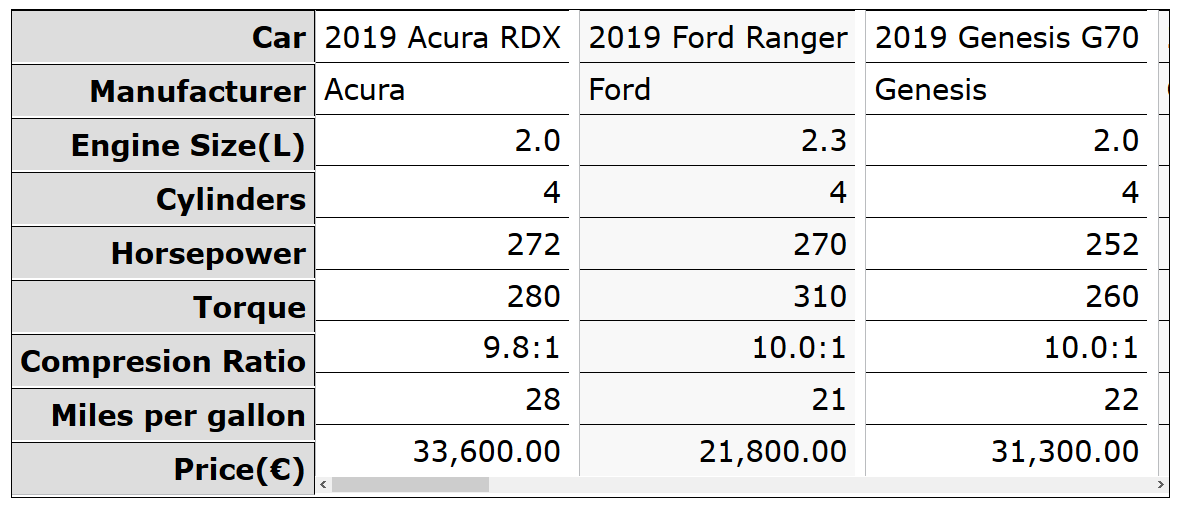
\includegraphics[width=1\linewidth]
    {images/flip_scroll.png}%
    \label{flip_scroll}%
    }


    \caption[Flip Scroll]
    {

    \imgcredit{Screenshot taken by the author.}
    }
    \label{figFlipScroll}
\end{figure}


\section{User Resizeable Columns}
This technique empowers the user quite significantly. As the title
suggests, the user is able to manipulate the size of a table's
columns. 

This technique is useful when the user is immune to space limitation
penalties the table might have on most other users. For example, if a
user has a screen big enough that space between columns is wasted to
keep column sizes consistent, being able to resize this column to
bring other columns into view is highly desireable.

User Resizeable Columns allows the user to tailor the table's
experience to his/her own preferences. 

There are two possible solutions. Both work for following browsers:
\begin{itemize}
    \item[--] Google Chrome
    \item[--] Mozzila Firefox
    \item[--] Internet Explorer
    \item[--] Opera
    \item[--] Microsoft Edge
\end{itemize}

Solution using only CSS and HTML:
\begin{lstlisting}[%
    language = HTML,
    xleftmargin=0cm,              % no extra margins for floats
    xrightmargin=0cm,             % no extra margins for floats
    language=biblatex,
    basicstyle=\footnotesize\ttfamily,
    frame=shadowbox,
    numbers=left,
    label=list:UserRColumns,
     stringstyle=\color{blue}
    ,
]
<thead>
    <tr>
        <th title="Car">
            <div class = "resizecell">Car</div>
        </th>
        <th title="Manufacturer">
            <div class = "resizecell">Manufacturer</div>
        </th>
        <th title="Engine Size(L)">
            <div class = "resizecell">Engine Size(L)</div>
        </th>
        [...]
    </tr>
</thead>
\end{lstlisting}

\begin{lstlisting}[%
    language = CSS,
    xleftmargin=0cm,              % no extra margins for floats
    xrightmargin=0cm,             % no extra margins for floats
    language=biblatex,
    basicstyle=\footnotesize\ttfamily,
    frame=shadowbox,
    numbers=left,
    label=list:URC2,
     stringstyle=\color{blue}
    ,
]
.resizecell {
    resize: horizontal;
    overflow: auto;
    width: 100%;
    hyphens: auto;
}
\end{lstlisting}

Encapsulating every header cell (or every single cell) with a
\texttt{$<$div$>$} tag allows CSS to enable resizeability by setting
the attribute \texttt{resize: horizontal} to these divs
\parencite{URC_1}.

Following image represents an HTML table with User Resizeable Columns
using only HTML and CSS:

\begin{figure}[tp]
    \centering

    {%
    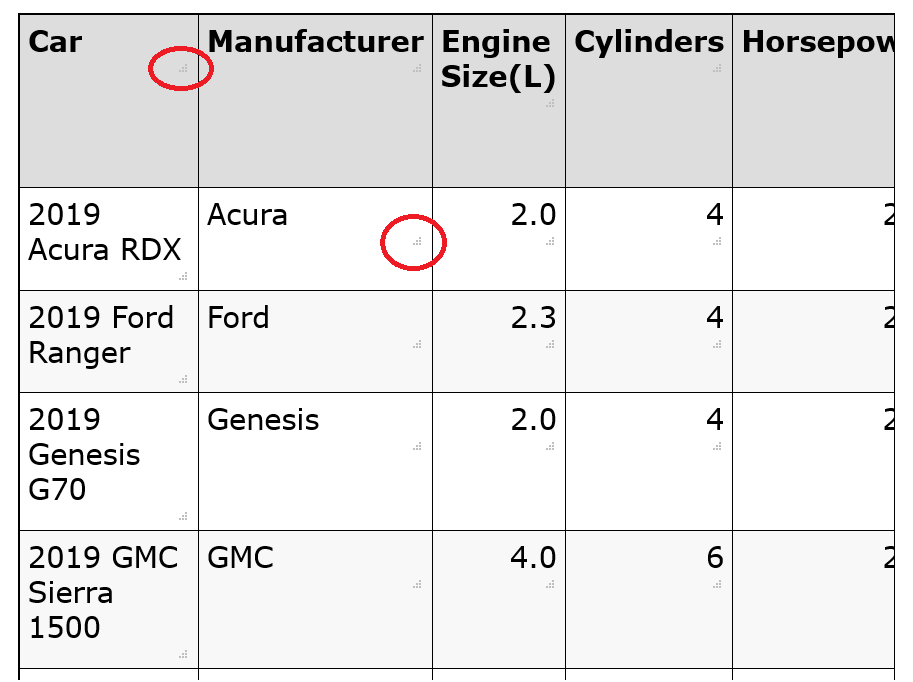
\includegraphics[width=1\linewidth]
    {images/urc_css.png}%
    \label{urc_css}%
    }


    \caption[User Resizeable Columns using only HTML and CSS]
    {

    \imgcredit{Screenshot taken by the author.}
    }
    \label{figURCCSS}
\end{figure}

Solution using JavaScript (jQuery):
\begin{lstlisting}[%
%    language = JavaScript,
    xleftmargin=0cm,              % no extra margins for floats
    xrightmargin=0cm,             % no extra margins for floats
    language=biblatex,
    basicstyle=\footnotesize\ttfamily,
    frame=shadowbox,
    numbers=left,
    label=list:UCR3,
     stringstyle=\color{blue}
    ,
]
~/js/jQuery.resizableColumns.js

$(function(){
  $('.rcl').resizeableColumns();
}); 
\end{lstlisting}

The trick is calling the \texttt{resizeableColumns()} on the table of
your choice \parencite{URC_2}.

\begin{figure}[tp]
    \centering

    {%
    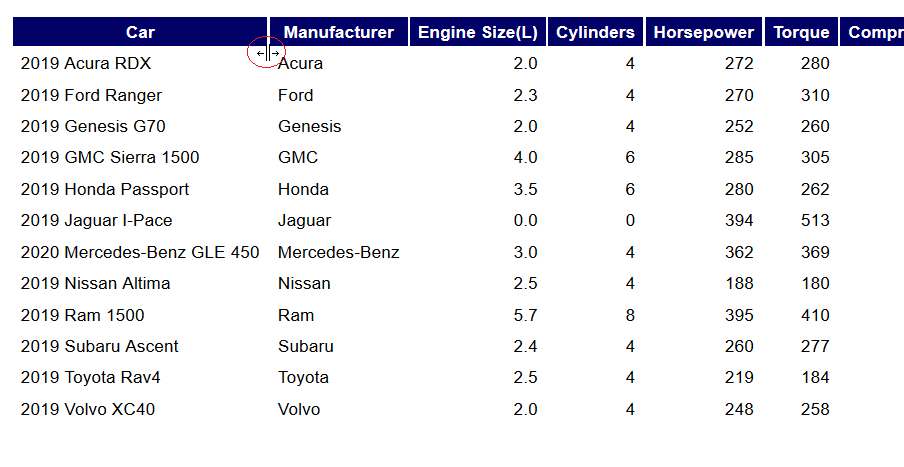
\includegraphics[width=1\linewidth]
    {images/urc_js.png}%
    \label{urc_js}%
    }


    \caption[User Resizeable Columns using JS (jQuery)]
    {

    \imgcredit{Screenshot taken by the author.}
    }
    \label{figURCJS}
\end{figure}

\section{Long Two Column}
Just like Flip Scroll, this technique is useful for an object-based
table; one where each row is populated by a single `object' where each
column represents a different feature of the object. 
\newline

Rather than having the user scroll through features, the user is now
able to scroll through objects vertically instead. This is the result
of transposing the table. The first column will now house the
(previously column) headers and the second column will house the data
previously housed in the first row. This creates a `minitable' for the
(previously) first row. For the next object (and row), another
`minitable' is created like with the first one and then appended
below. This approach creates a `minitable' for each object and appends
it to the previous object. 

As the name suggest, you end up with a long table of 2 columns, the
first of which is 'always the same'.

Unlike Flip scroll, it does not keep the table in the allocated space,
unless you set vertical scrolling.

This solution works for following browsers:\begin{itemize}
    \item[--] Google Chrome
    \item[--] Mozzila Firefox
    \item[--] Internet Explorer
    \item[--] Opera
    \item[--] Microsoft Edge
\end{itemize}

\begin{lstlisting}[%
    language = CSS,
    xleftmargin=0cm,              % no extra margins for floats
    xrightmargin=0cm,             % no extra margins for floats
    language=biblatex,
    basicstyle=\footnotesize\ttfamily,
    frame=shadowbox,
    numbers=left,
    label=list:LongTwoColumn,
     stringstyle=\color{blue}
    ,
]
table, thead, tbody, th, td, tr {
    display: block;
}

td {
    /* Behave  like a "row" */
    border: none;
    border-bottom: 0.0625rem solid #eee;
    position: relative;
    padding-left: 50%;
}

td:before {
    /* Now like a table header */
    position: absolute;
    /* Top/left values mimic padding */
    top: 0;
    left: 0.375rem;
    width: 45%;
    padding-right: 0.625rem;
    white-space: nowrap;
}
\end{lstlisting}

The trick is setting the table's elements to
 \texttt{display: block} and the $<$\texttt{td}$>$ 
 tag's attribute to \texttt{position: relative} \parencite{L2C}.

Following image represents an HTML table with Long Two Column:

\begin{figure}[tp]
    \centering

    {%
    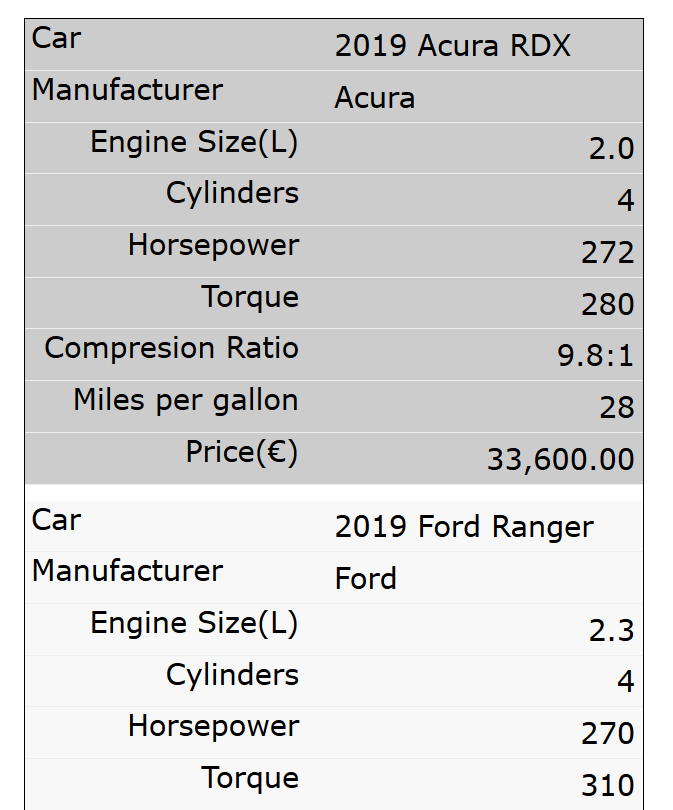
\includegraphics[width=0.65\linewidth]
    {images/long_two_column.png}%
    \label{long_two_column}%
    }


    \caption[Long Two Column] 
    {

    \imgcredit{Screenshot taken by the author.}
    }
    \label{figLongTwoColumn}
\end{figure}


\cleardoublepage
%----------------------------------------------------------------
%
%  File    :  survey-recc.tex
%
%  Author  :  Mirza Kabiljagic, Stefan Rajinovic, Aleksandar Stojicic,
%             Inti Gabriel Mendoza Estrada
%
%  Created :  27 May 20xx
%
%  Changed :  4 Dez 2019
%
%----------------------------------------------------------------


\chapter{Recommendation}
\label{chap:Recommendation}
 


\section{Recommendation}

Responsive tables must be able to efficiently and effectively display data. It is only through a combination of good table design and responsive techniques one is able to achieve this. 

For good table design, it is imperative that you include Alternate Row Highlighting. This is a very simple technique that works on every browser and is not only helpful to the user but to the developer as it adds positively to the aesthetics. 

For a ``Jack of all trades'' approach, we suggest the following responsive techniques: Long Two Column, and Fixed Header. You are able to apply this for the 3 main screen sizes: PC, tablet, and phone. Being able to apply Long Two Column to phone-sized screens (or tablets in vertical mode) and leave Fixed Header on the remaining two sizes (PC and tablets in horizontal mode) automatically eliminates one of the 3 sizes you have to take care of. 

Another thing to keep in mind is to attach the vertical scrollable feature of Fixed Header to the Long Two Column. This ensures that the space the table is taking up is exactly the one allocated to it. It goes without saying that if the table is too wide (horizontally), it should be horizontally scrollable.

The figure below shows these techniques working together.

\begin{figure}[tp]
    \centering
  
    {%
    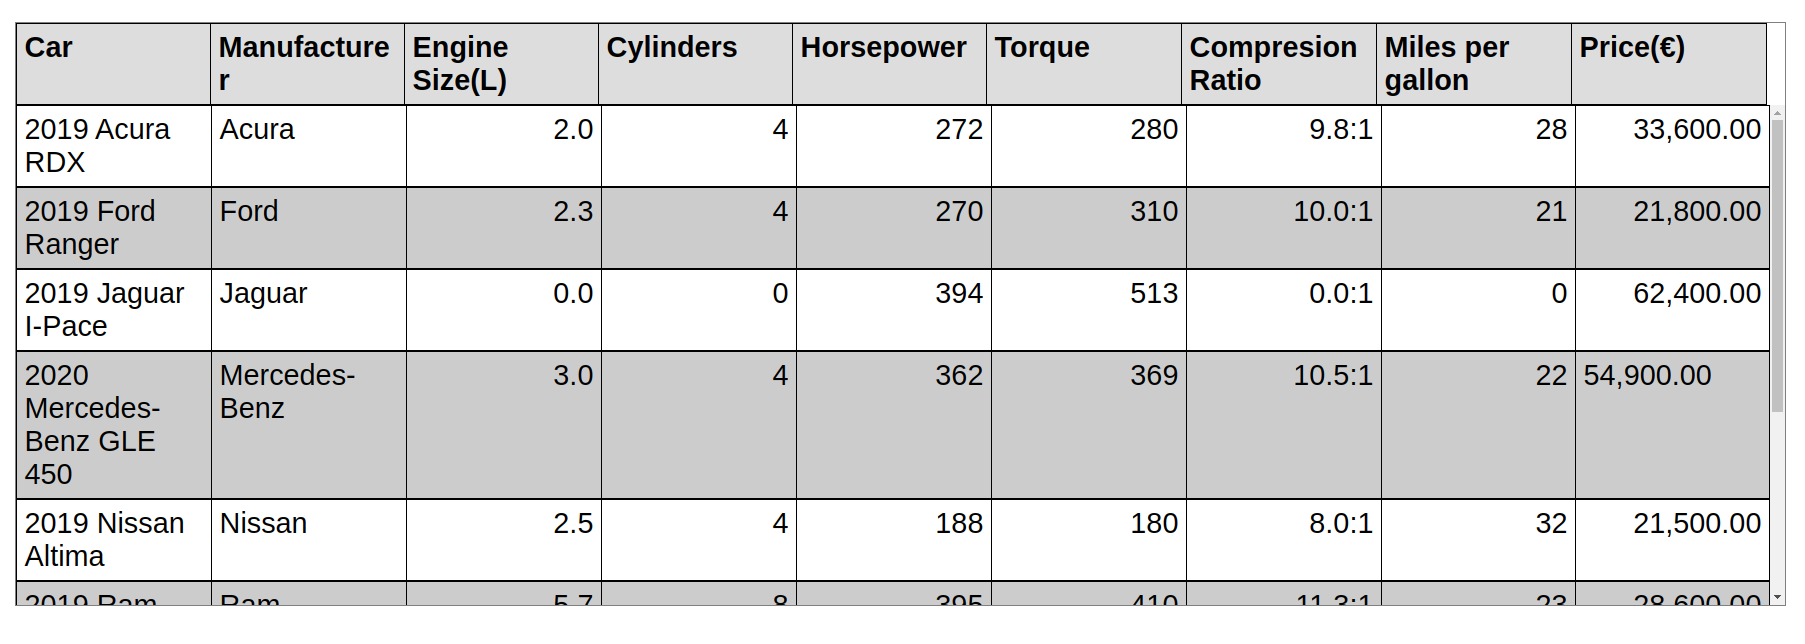
\includegraphics[width=1\linewidth]
    {images/recommendation_1.png}%
    \label{Recommendation 1}%
    }

    
    \caption[Recommendation Techniques 1]
    {
      
    \imgcredit{Screenshot taken by the author.}
    }
    \label{figRecc1}
\end{figure}

As you scroll through the table, notice the Fixed Header Technique in the image below.

\begin{figure}[tp]
    \centering
  
    {%
    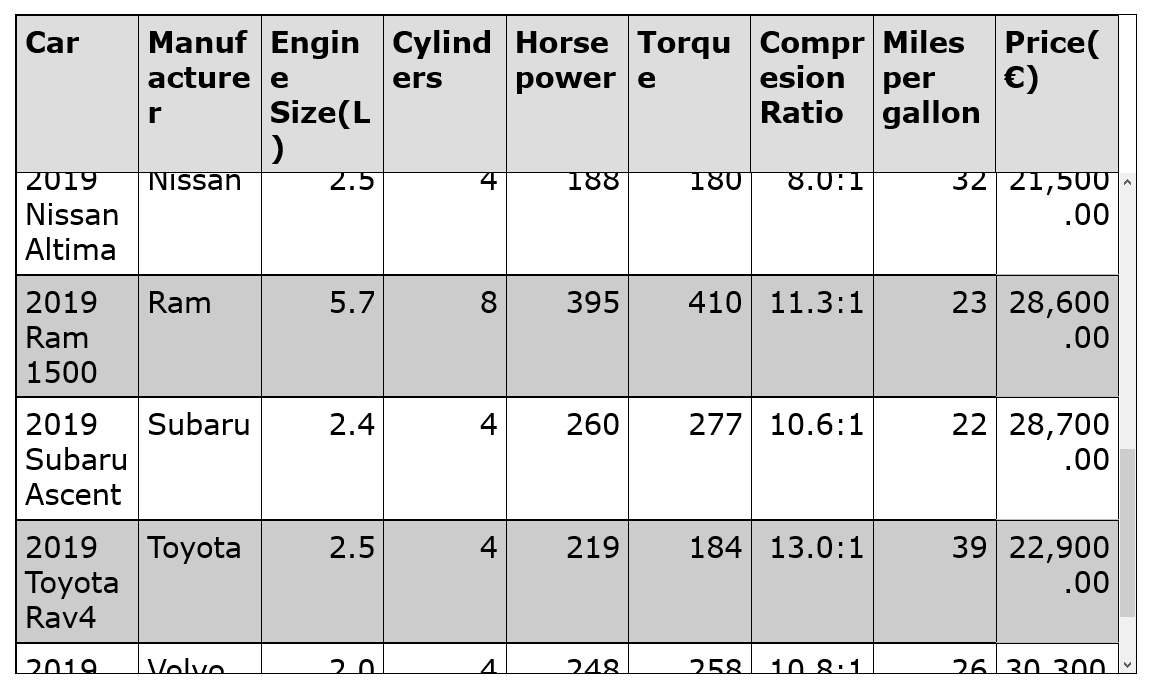
\includegraphics[width=1\linewidth]
    {images/recommendation_2.png}%
    \label{Recommendation 2}%
    }

    
    \caption[Recommendation Techniques 2]
    {
      
    \imgcredit{Screenshot taken by the author.}
    }
    \label{figRecc2}
\end{figure}

For small-sized screens, the technique that would ``kick in'' is shown in the image below. Notice the `creeping' second `minitable' in the bottom part.

\begin{figure}[tp]
    \centering
  
    {%
    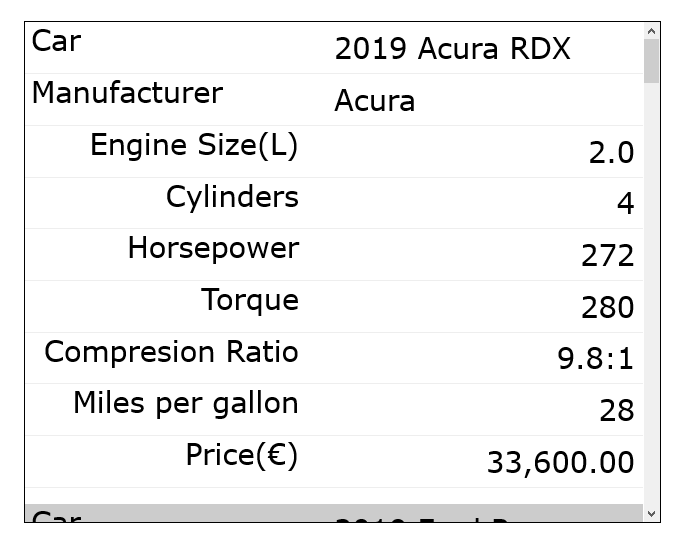
\includegraphics[width=1\linewidth]
    {images/recommendation_3.png}%
    \label{Recommendation 3}%
    }

    
    \caption[Recommendation Techniques 3]
    {
      
    \imgcredit{Screenshot taken by the author.}
    }
    \label{figRecc3}
\end{figure}






\cleardoublepage
% for now, switch to language english
% hack to force unix date for biblio, biblatex 3.11
\begin{otherlanguage}{english}
\printbibliography[heading=bibintoc]
\end{otherlanguage}


\end{document}